%%%%%%%%%%%%%%%%%%%%%%%%%%%%%%%%
% Chap 2. Related works of action recognition
%%%%%%%%%%%%%%%%%%%%%%%%%%%%%%%%

\chapter{Preliminaries}\label{chapter2}
%1차 수정 완료
Synchronous Machines (SMs) generate electrical torque through the continuous interaction of the two rotating magnetic fields, which are generated by the stator and the rotor, so it is important to analyze the physical behavior of the stator flux linkage. In Section \ref{chap2:2.1}, the basic physical characteristics and mathematical model of SM are briefly reviewed. In general, stator flux linkage can be expressed as a nonlinear function of stator current and machine parameters, so the voltage equation of SM can be represented by the dynamics of the stator current. Therefore, current control methods for SM based on stator current dynamics are briefly introduced in Section \ref{chap2:2.2}. To properly perform these methods, accurate parameter information, such as inductances and permanent magnet flux linkages, is required. However, these parameters vary nonlinearly with the stator current and the temperature of the stator windings and rotor, affecting the control performance of the SM. Thus, Section \ref{chap2:2.3} introduces conventional approaches for online stator flux linkage estimation, which is the first step in obtaining the parameters required for current control or optimal torque control.

\section{Mathematical Model of SM}\label{chap2:2.1}
\subsubsection{Modeling in the ($a$,$b$,$c$)-reference frame}
In SM, each stator winding in the ($a$,$b$,$c$)-reference frame is connected in a Y-connection structure, and according to Kirchhoff's law, the sum of all instantaneous stator currents is zero, i.e. 
\begin{equation}\label{eqn:2.1}
i^a_s(t)+i^b_s(t)+i^c_s(t)=0, \quad \forall t \geq 0    
\end{equation}
where the voltage applied to the three-phase stator windings of an SM consists of the voltage drop across the winding resistance and the induced voltage due to the time derivative of the stator flux linkage, as described by Faraday’s law. Therefore, the mathematical model of the SM can be expressed as
\begin{equation}\label{eqn:2.2}
\mathbf{u}^{abc}_s(t) = R_s \mathbf{i}^{abc}_s(t) + \frac{d}{dt}\underbrace{\bm{\psi}^{abc}_s \left( \mathbf{i}^{abc}_s(t),\theta_r(t)\right)}_{=:\bm{\psi}^{abc}_s(t)},
\end{equation}
\begin{equation}\notag
\left(
    \theta_r(t) := n_p(\theta_m(t) + \theta_{pm})=n_p\left( \int_0^t \omega_m(\tau)d\tau + \theta_{pm}\right)
    \right)
\end{equation}
\begin{figure}[t]
    \centering
    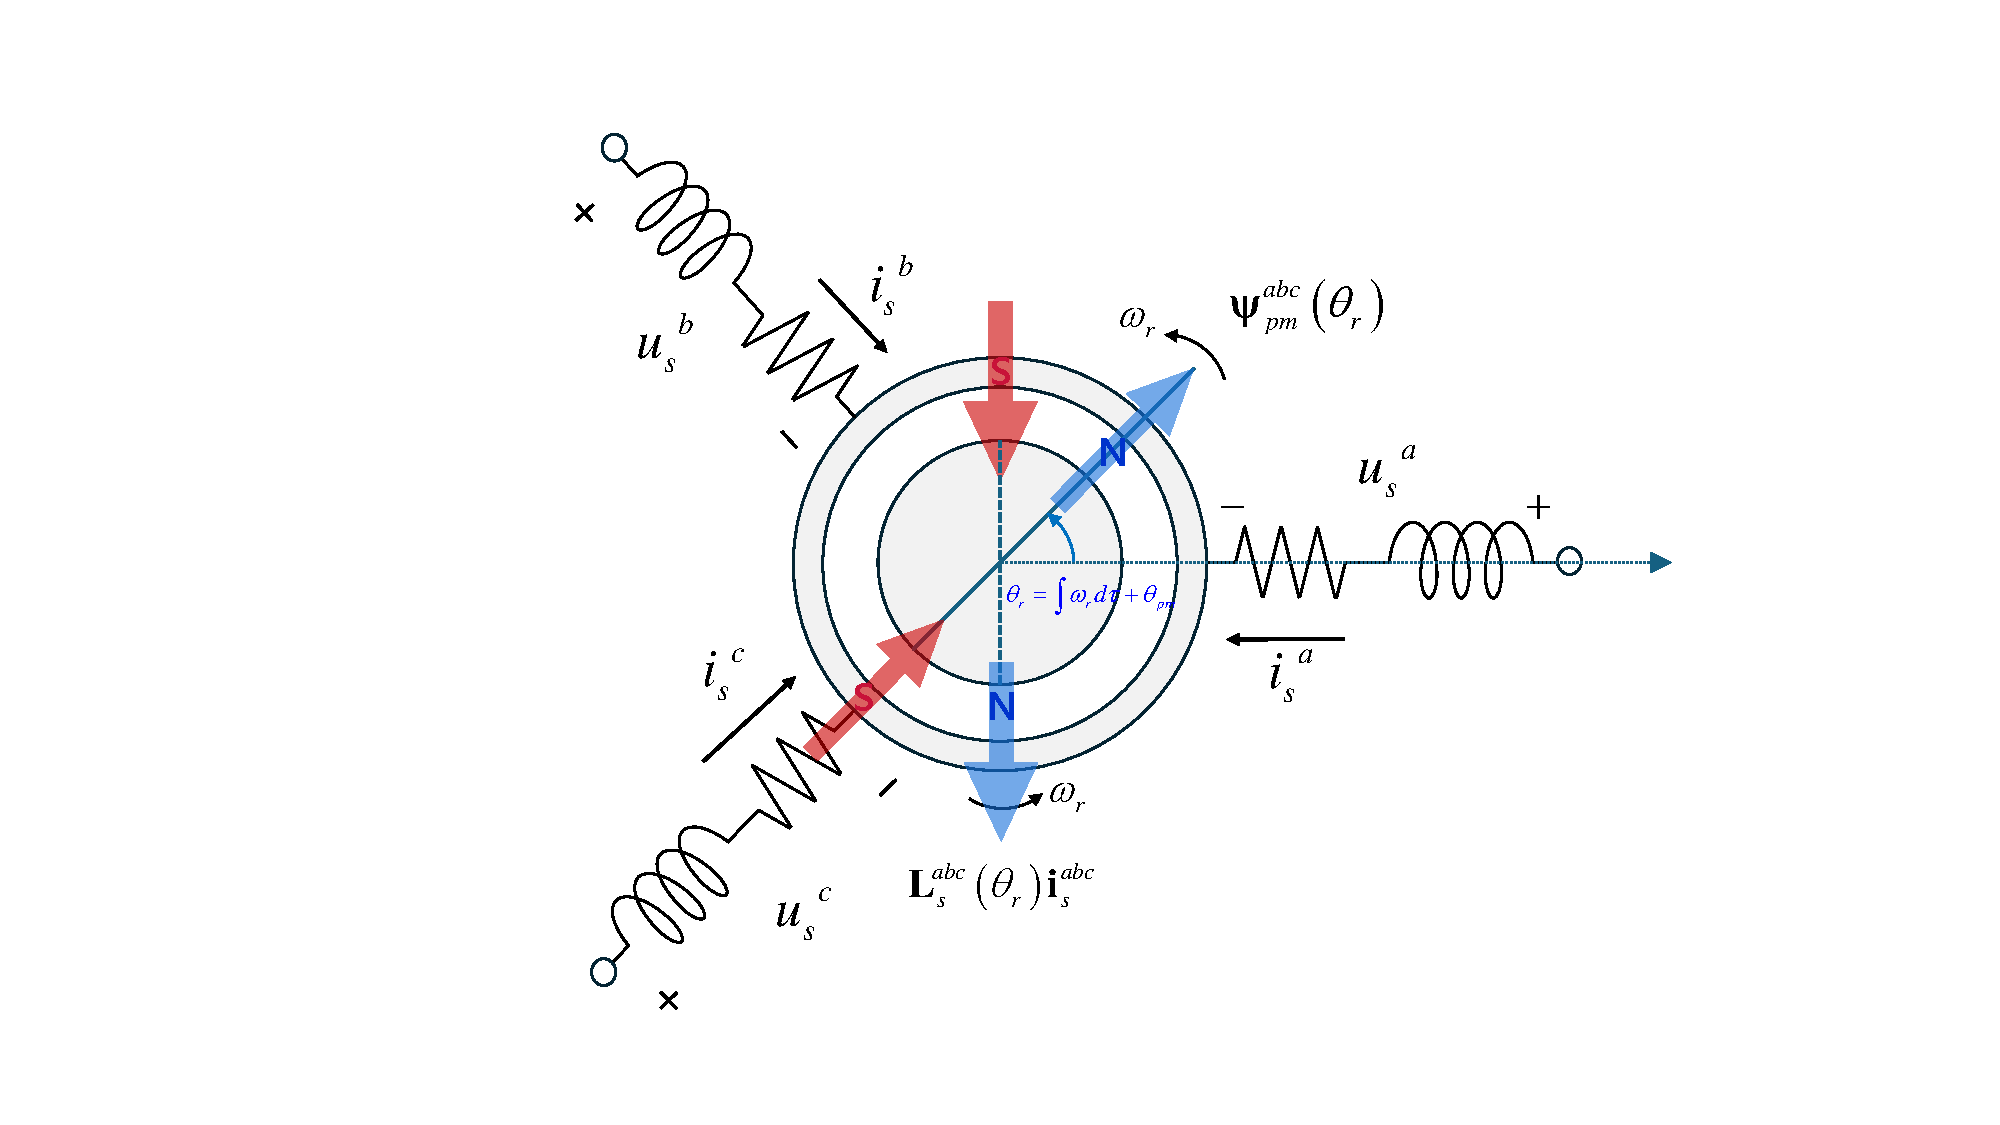
\includegraphics[scale=0.52]{chapters/Fig2.1.pdf}
    \caption{SM structure.}
    \label{Fig:2.1}
\end{figure}
where $R_s$ is the stator resistance, $\mathbf{u}^{abc}_{s} := (u^a_s, u^b_s, u^c_s)^\top$ $(\text{in } \mathbf{V} \cdot \mathbb{R}^3)$ and $\mathbf{i}^{abc}_s := (i^a_s, i^b_s, i^c_s)^\top$ $(\text{in } \mathbf{A} \cdot \mathbb{R}^3)$ denote the \emph{stator phase voltages} and \emph{stator phase currents} in the phase windings, respectively.  The linear combination of the magnetic fields produced by the phase currents and the permanent magnets in the rotor (if present) yields the \emph{overall stator flux linkages} $\boldsymbol{\psi}^{abc}_s:= (\psi^a_s, \psi^b_s, \psi^c_s)^\top$ $(\text{in } \mathbf{Wb} \cdot \mathbb{R}^3)$. $\theta_r$ and $\theta_m$ $(\text{in rad})$ denote the electrical and mechanical rotor position between the $d$-axis and the $as$-axis, which changes over time and $\theta_{pm}$ (in rad) is an orientation offset (constant) of the permanent magnets concerning the axis of phase $a$ (see Fig.\ref{Fig:2.1}). $\omega_m$ (in rad/s) is the mechanical angular velocity and  $n_p$ $(\in \mathbb{N})$ denotes the pole pair number.

As an exemplary model of a synchronous machine, the stator flux linkage vector of a synchronous machine with embedded permanent magnets in the rotor (interior permanent magnet synchronous machine, $\textbf{IPMSM}$) is given by (see Chap.5 in \cite{c2.1_1})
\begin{align}\notag
\boldsymbol{\psi}^{abc}_s\left( \mathbf{i}^{abc}_s,\theta_r\right) &= \underbrace{\begin{bmatrix}
    L^{aa}_s & L^{ab}_s & L^{ac}_s \\
    L^{ba}_s & L^{bb}_s & L^{bc}_s\\
    L^{ca}_s & L^{cb}_s & L^{cc}_s
\end{bmatrix}}_{=:\mathbf{L}^{abc}_s(\theta_r) \in \mathbb{R}^{3\times3}}\mathbf{i}^{abc}_{s} + \underbrace{\psi_{pm}\begin{bmatrix}
\cos \theta_r \\ \cos \left( \theta_r - \frac{2\pi}{3} \right) 
\\
\cos \left( \theta_r + \frac{2\pi}{3} \right)
\end{bmatrix}}_{=:\boldsymbol{\psi}^{abc}_{pm}(\theta_r)\in \mathbb{R}^{3}}\\\label{eqn:2.3}
&= \mathbf{L}^{abc}_s(\theta_r)\mathbf{i}^{abc}_{s}+\boldsymbol{\psi}^{abc}_{pm}(\theta_r),
\end{align}
in the ($a$,$b$,$c$)-reference frame with the stator inductance matrix
\begin{equation}\notag
\small
 \mathbf{L}^{abc}_s(\theta_r) := \begin{bmatrix}
L_{ls} + L_A - L_B \cos 2\theta_r & -\frac{1}{2} L_A + L_B \cos 2 \left( \theta_r - \frac{\pi}{3} \right) & -\frac{1}{2} L_A + L_B \cos 2 \left( \theta_r + \frac{\pi}{3} \right) \\
-\frac{1}{2} L_A + L_B \cos 2 \left( \theta_r - \frac{\pi}{3} \right) & L_{ls} + L_A - L_B \cos 2 \left( \theta_r + \frac{\pi}{3} \right) & -\frac{1}{2} L_A + L_B \cos 2\theta_r \\
-\frac{1}{2} L_A + L_B \cos 2 \left( \theta_r + \frac{\pi}{3} \right) & -\frac{1}{2} L_A + L_B \cos 2\theta_r & L_{ls} + L_A - L_B \cos 2 \left( \theta_r - \frac{\pi}{3} \right)
\end{bmatrix},    
\end{equation}
where $\mathbf{L}^{abc}_s$ (in $\mathbf{H=Vs/A} \cdot \mathbb{R}^{3\times3}$) is a position-dependent stator inductance matrix in the ($a$,$b$,$c$)-reference frame, where the diagonal elements denote the self-inductance, and the off-diagonal elements represent the mutual inductance. $\boldsymbol{\psi}^{abc}_{pm}$ (in $\mathbf{Wb} \cdot \mathbb{R}^{3}$) is a position-dependent \emph{permanent-magnet flux linkage vector} with a magnitude of $\psi_{pm}$. \(L_{ls}\) is the leakage inductance of the stator windings, \(L_A\) is the inductance independent of the rotor's position, and \(L_B\) is the maximum inductance that varies with rotation due to the salient rotor structure. The structure of SM and an example of the phase $as$ winding stator inductance in IPMSM are illustrated in Fig.\ref{Fig:2.1} and Fig.\ref{Fig:2.2}, respectively. 

According to equation (\ref{eqn:2.1}), if all physical signals of the three-phase winding are balanced, one physical quantity can be expressed in terms of the other two ($i^a_s(t)=-i^b_s(t)-i^c_s(t), \forall t \geq 0$). Consequently, using reference frame transformations with matrix equations, the physical quantities in the ($a$,$b$,$c$)-reference frame can be projected into either the stationary ($\alpha$,$\beta$)-reference frame or the synchronously rotating ($d$,$q$)-reference frame, which can simplify three physical quantities into two. Figure \ref{Fig:2.3} shows the reference frame transformation according to each frame.
\begin{figure}[t]
    \centering
    \begin{subfigure}[b]{0.45\textwidth}
        \centering
        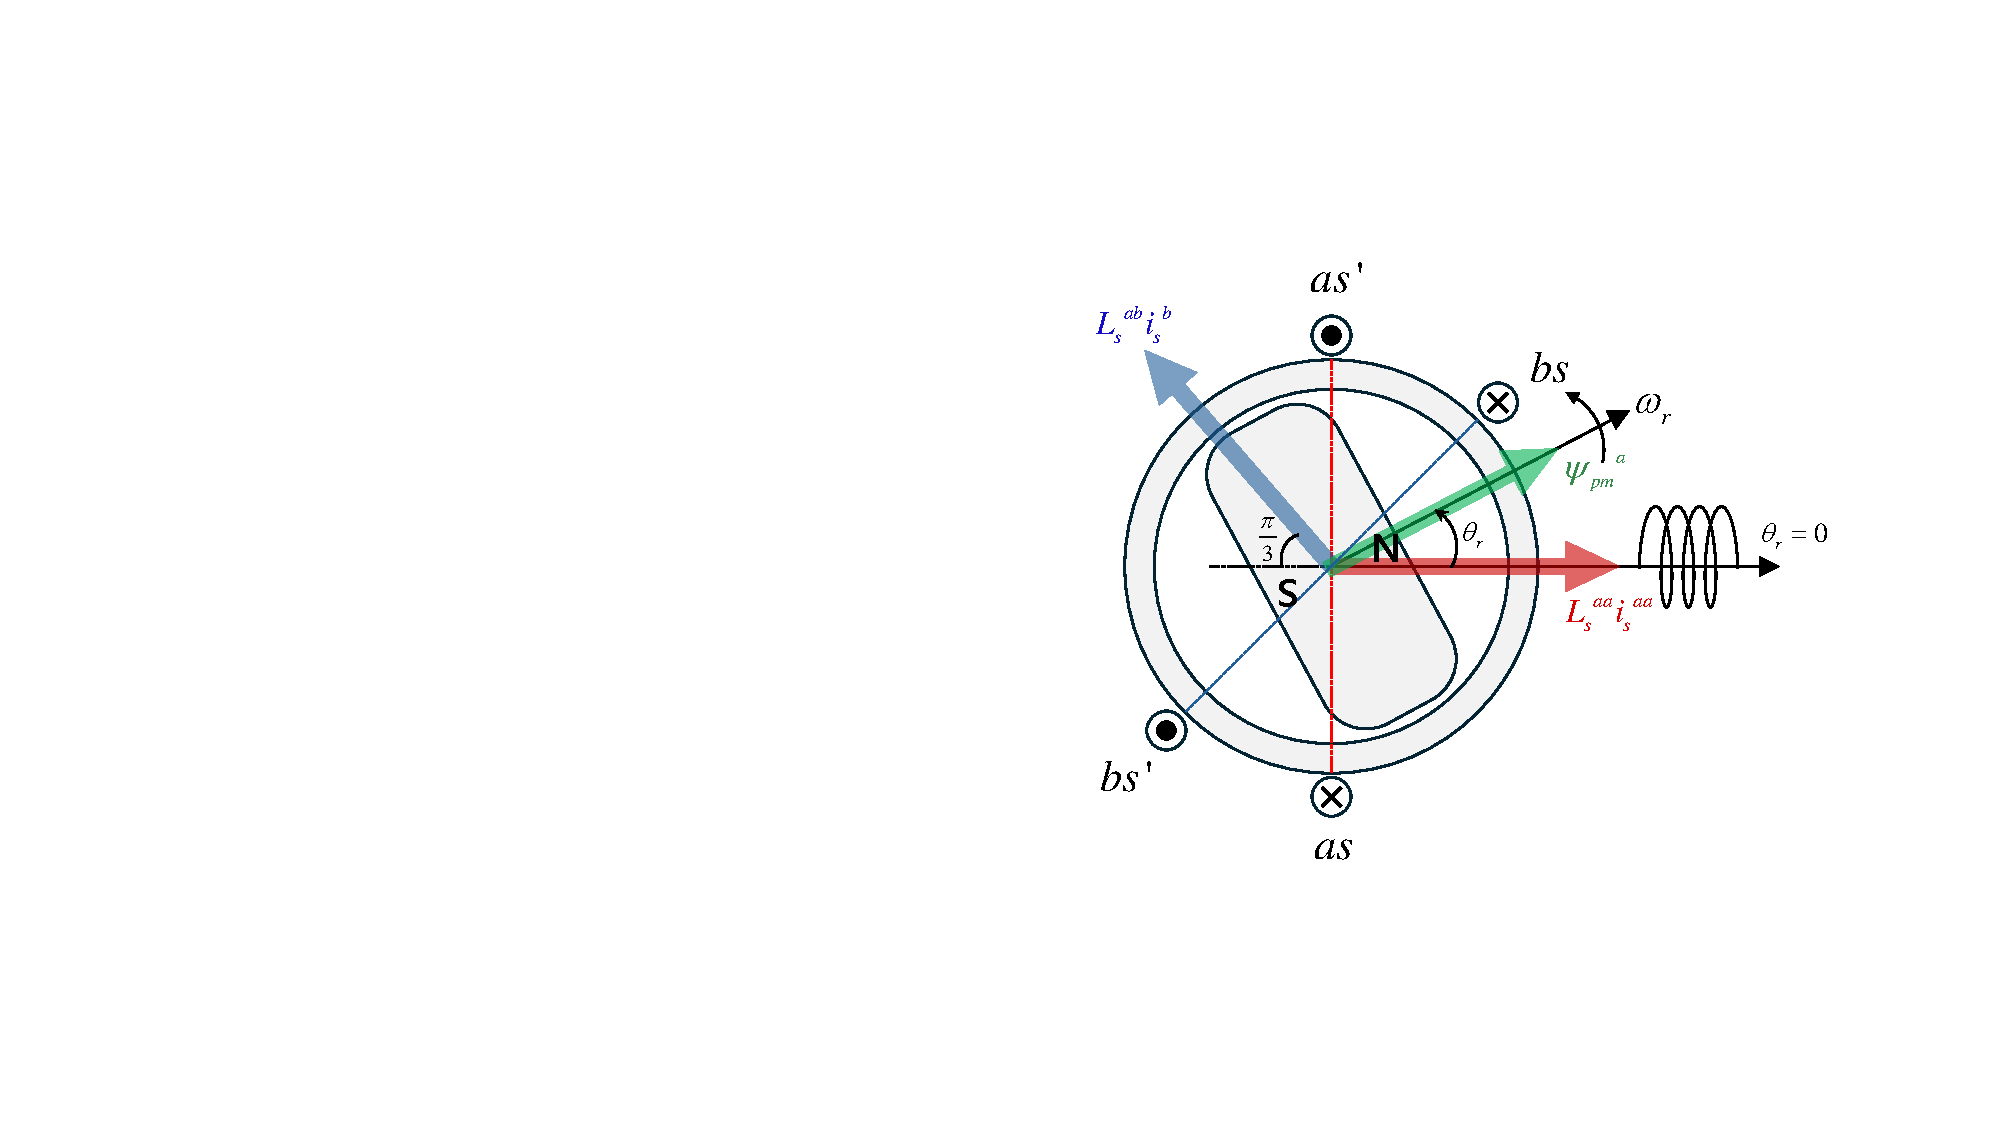
\includegraphics[scale=0.6]{chapters/Fig2.2a.pdf}
        \caption{}
        \label{Fig:2.2a}
    \end{subfigure}
    \hfill
    \begin{subfigure}[b]{0.45\textwidth}
        \centering
        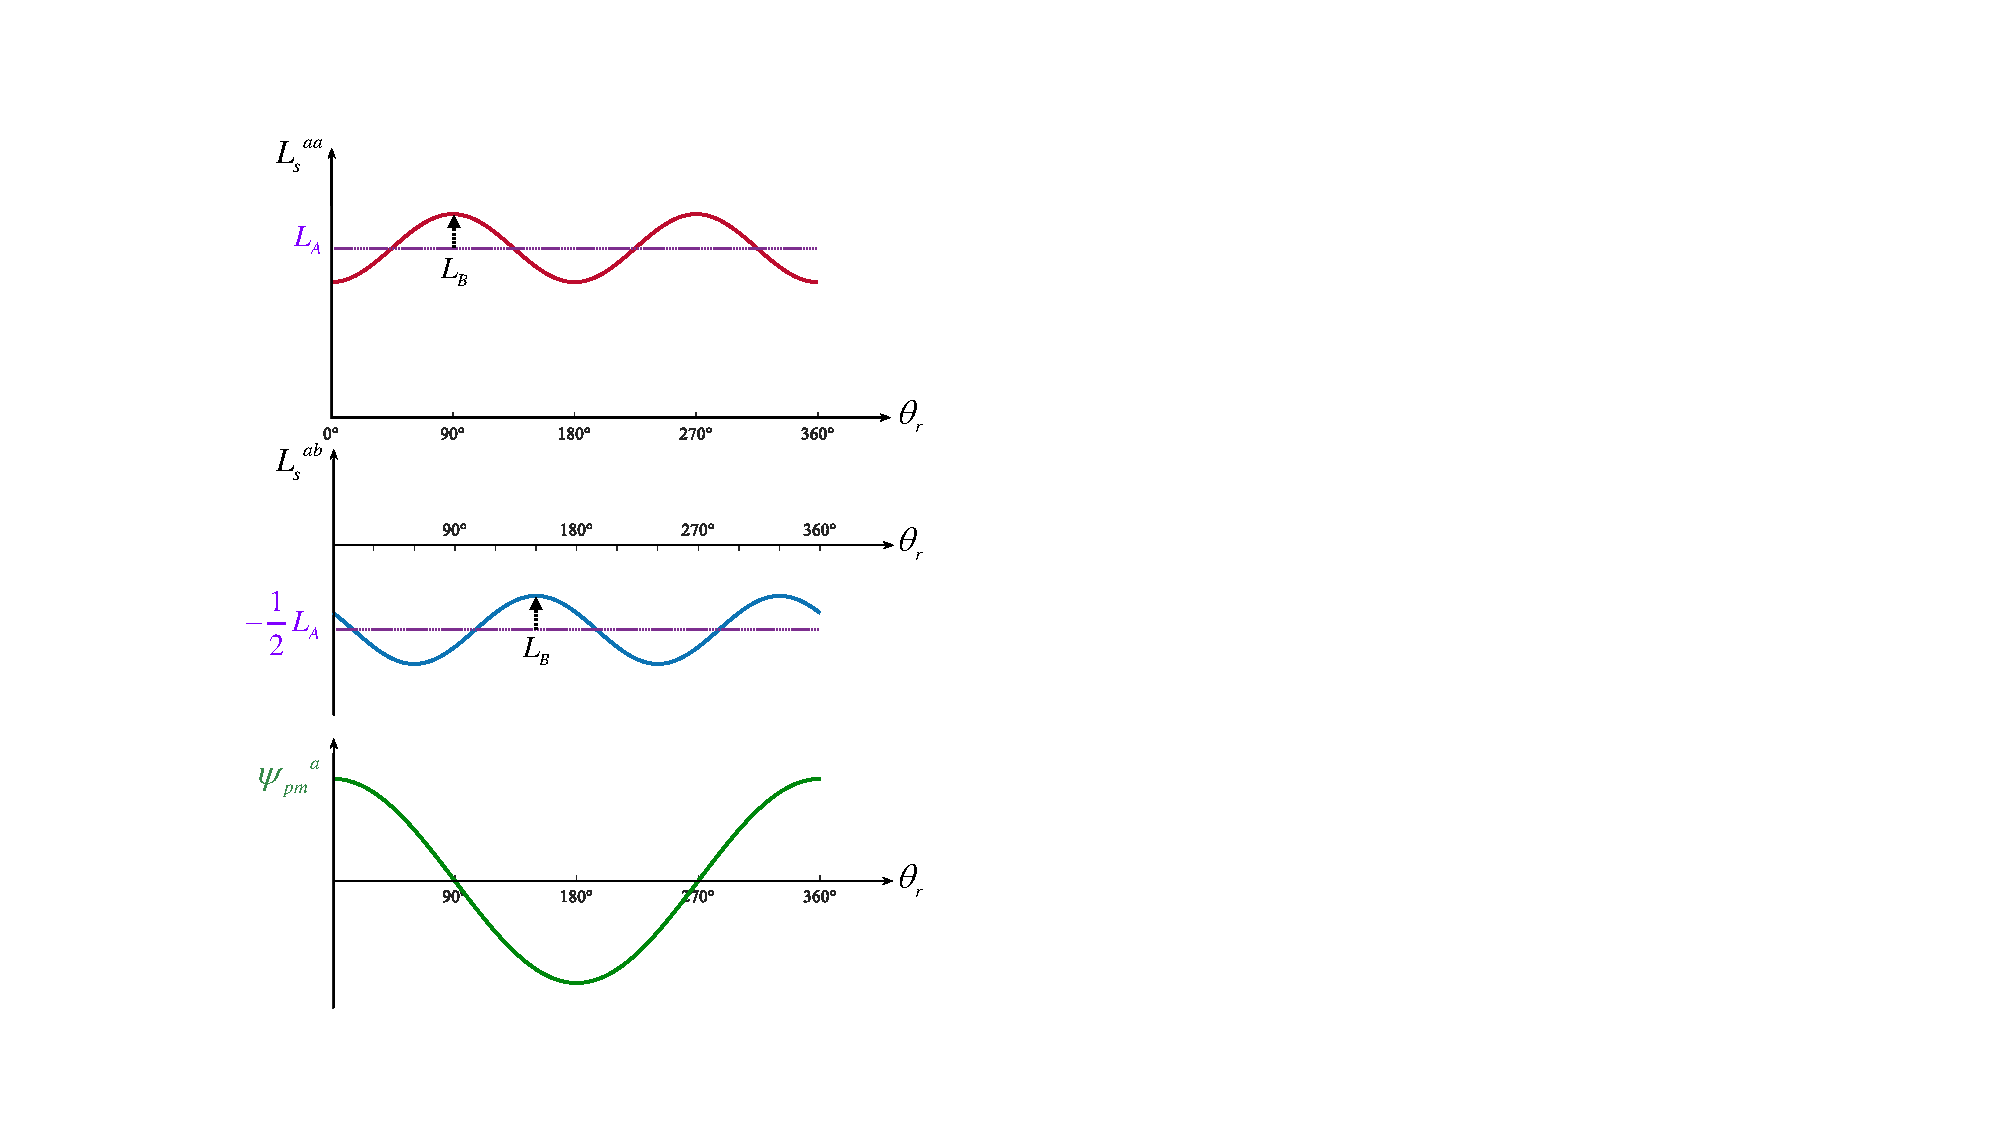
\includegraphics[scale=0.6]{chapters/Fig2.2b.pdf}
        \caption{}
        \label{Fig:2.2b}
    \end{subfigure}
    \caption{The stator inductance of phase $as$ winding for rotor positions. (a) magnetic equivalent rotor and flux linkages of an IPMSM. (b) in order, the self-inductance of the stator $as$ winding, the mutual inductance between $as$ and $bs$ phases, and the inductance between the stator $as$ winding and the magnet.}
    \label{Fig:2.2}
\end{figure}
\begin{figure}[t]
    \centering
    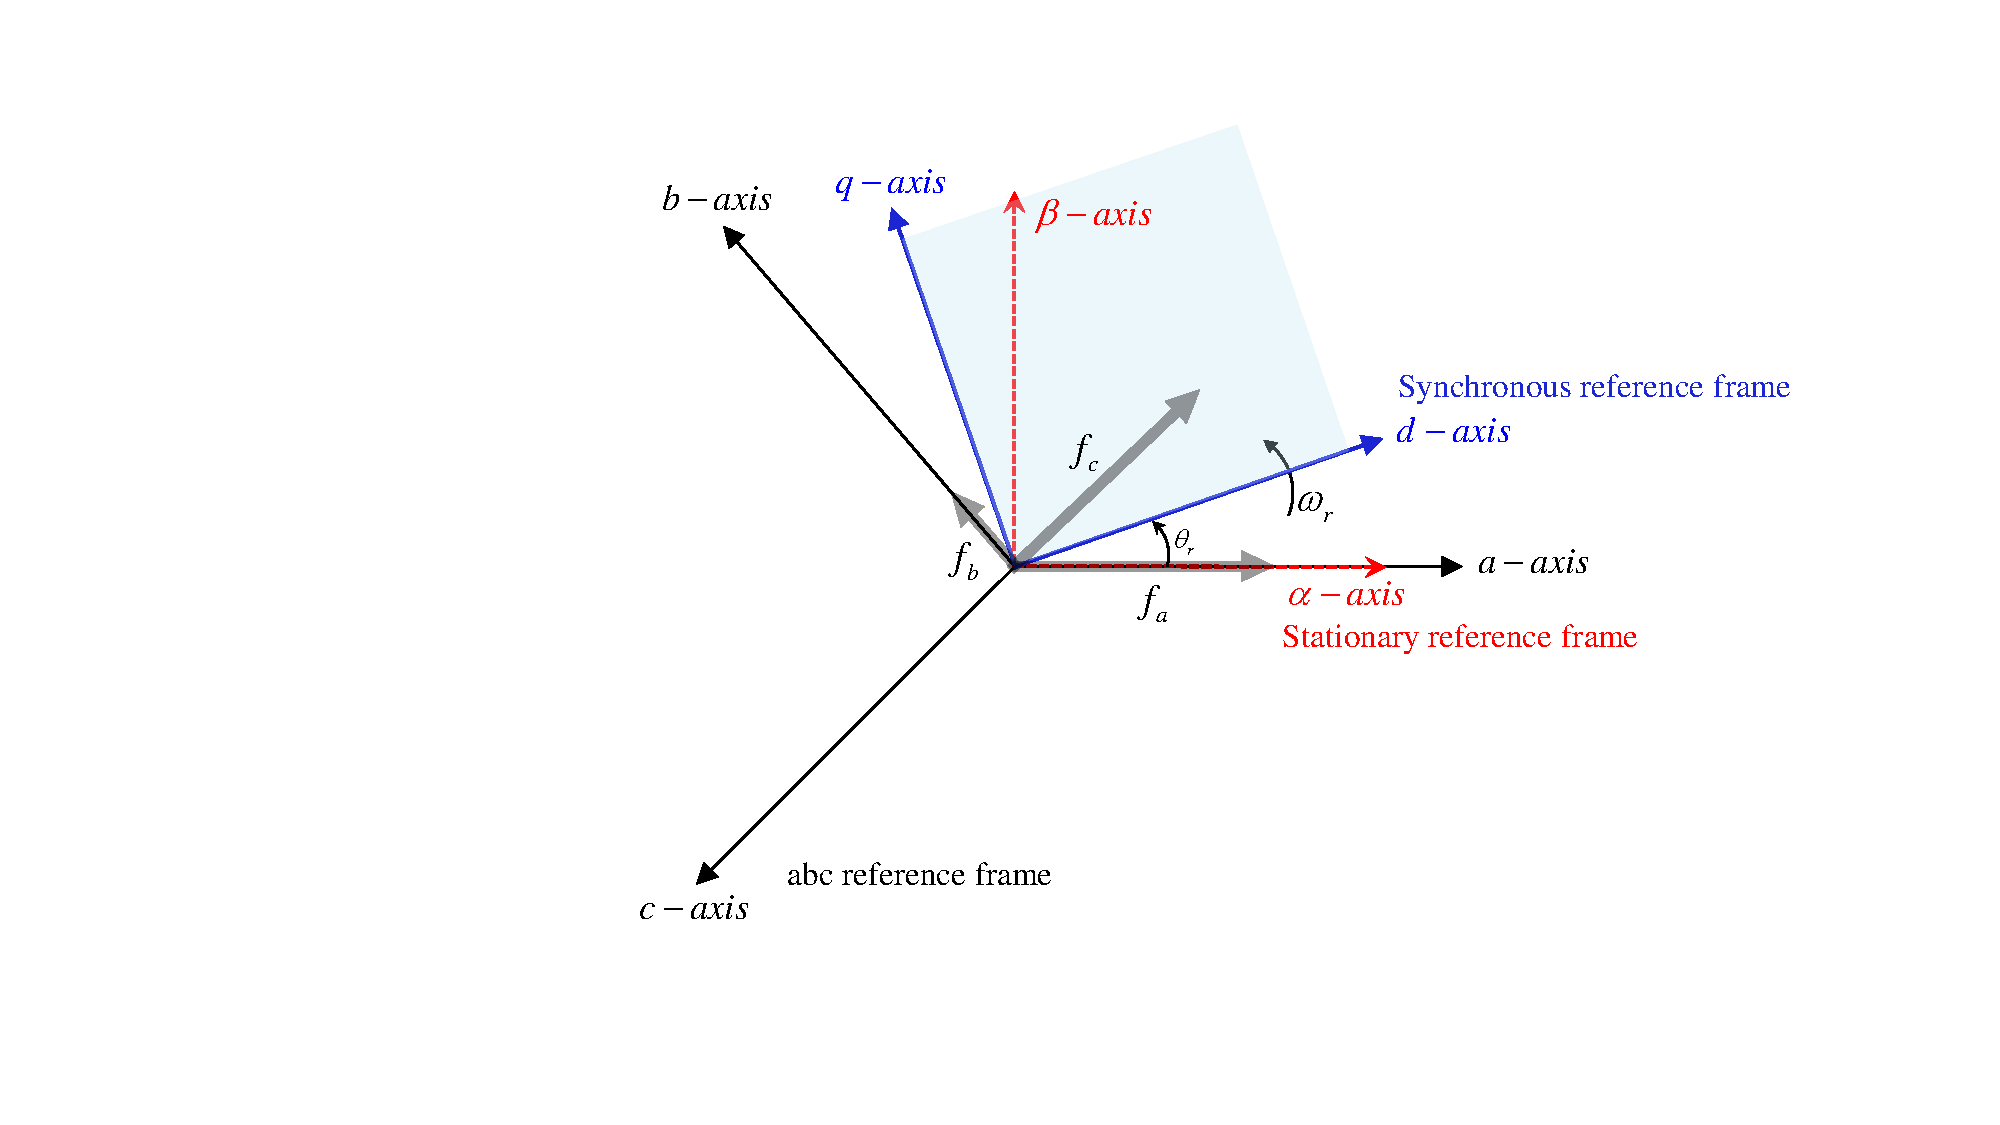
\includegraphics[scale=0.6]{chapters/Fig2.3.pdf}
    \caption{($a$,$b$,$c$)-reference frame, stationary ($\alpha$,$\beta$)-reference frame and rotating ($d$,$q$)-reference frame.}
    \label{Fig:2.3}
\end{figure}

\subsubsection{Modeling in the stationary  ($\alpha$,$\beta$)-reference frame}
The machine model (\ref{eqn:2.2}) can be expressed in the stationary ($\alpha$,$\beta$)-reference frame with orthogonal $\alpha$- and $\beta$-axes, where the zero-sequence component can be neglected due to the balanced three-phase signals in (\ref{eqn:2.1}). Such stator-fixed reference frame transformation for balanced signals can be simplified by using the transformation matrix
\begin{equation}\label{eqn:2.4}
\mathbf{T}(0) := \underbrace{\frac{2}{3} \begin{bmatrix}
1 & -\frac{1}{2} & -\frac{1}{2} \\
0 & \frac{\sqrt{3}}{2} & -\frac{\sqrt{3}}{2}\\
\frac{1}{2} & \frac{1}{2} & \frac{1}{2}
\end{bmatrix}}_{\mathbf{T}(0)\in \mathbb{R}^{3\times3}} \Rightarrow 
\mathbf{T}_c := \underbrace{\frac{2}{3} \begin{bmatrix}
1 & -\frac{1}{2} & -\frac{1}{2} \\
0 & \frac{\sqrt{3}}{2} & -\frac{\sqrt{3}}{2} 
\end{bmatrix}}_{\mathbf{T}_c\in \mathbb{R}^{2\times3}},
\end{equation}
where $\mathbf{T}(0)$ is called the \emph{Clarke transformation matrix} and $\mathbf{T}_c$ represents the \emph{simplified Clarke transformation matrix}, where the last row in $\mathbf{T}(0)$ can be neglected for balanced signals (see Chap.14 in \cite{c2.1_3}), reducing the three-phase signal vectors to two. By introducing the transformed quantities 
\begin{equation}\notag
\bm{u}_s^{\alpha\beta} := \mathbf{T}_c \bm{u}_s^{abc}, \quad \bm{i}_s^{\alpha\beta} := \mathbf{T}_c \bm{i}_s^{abc}, \quad \bm{\psi}_s^{\alpha\beta} := \mathbf{T}_c \bm{\psi}_s^{abc} \quad \text{and} \quad \mathbf{T}_c \frac{d}{dt} \bm{\psi}_s^{abc} = \frac{d}{dt} \bm{\psi}_s^{\alpha\beta}
\end{equation}
in the ($\alpha$,$\beta$)-reference frame and the machine dynamics in (\ref{eqn:2.2}) can be expressed as 
\begin{align}\label{eqn:2.5}\notag
\mathbf{u}^{\alpha\beta}_s(t) &= \mathbf{T}_c \mathbf{u}^{abc}_s(t) \\
&= R_s \mathbf{i}^{\alpha\beta}_s(t) + \frac{d}{dt}\underbrace{\bm{\psi}^{\alpha\beta}_s\left(\mathbf{i}^{\alpha\beta}_s(t),\theta_r(t) \right)}_{=:\bm{\psi}^{\alpha\beta}_s(t)},
\end{align}
where $\mathbf{u}^{\alpha\beta}_s := (u^\alpha_s, v^\beta_s)^\top$, $\mathbf{i}^{\alpha\beta}_s := (i^\alpha_s, i^\beta_s)^\top$ and $\bm{\psi}^{\alpha\beta}_s := (\psi^\alpha_s, \psi^\beta_s)^\top$ denote the stator voltage, current and flux linkage vectors in the ($\alpha$,$\beta$)-reference frame, respectively. 

Likewise, applying the simplified clarke transformation in (\ref{eqn:2.4}) to the stator flux linkage vector in (\ref{eqn:2.3}) yields the stator flux linkage vector
\begin{align}\label{eqn:2.7}\notag
\boldsymbol{\psi}^{\alpha\beta}_s\left(\mathbf{i}^{\alpha\beta}_s,\theta_r \right) &= \mathbf{T}_c\boldsymbol{\psi}^{abc}_s\left(\mathbf{i}^{abc}_s,\theta_r \right) \\\notag
&= \underbrace{\mathbf{T}_c\mathbf{L}^{abc}_s(\theta_r)\mathbf{T}^{-1}_c}_{=:\mathbf{L}^{\alpha\beta}_s(\theta_r)\in \mathbb{R}^{2\times2}}\mathbf{i}^{\alpha\beta}_s+\underbrace{\mathbf{T}_c\boldsymbol{\psi}^{abc}_{pm}(\theta_r)}_{=:\boldsymbol{\psi}^{\alpha\beta}_{pm}(\theta_r)\in \mathbb{R}^{2}}
\\
&= \mathbf{L}^{\alpha\beta}_s(\theta_r)\mathbf{i}^{\alpha\beta}_s
+ \boldsymbol{\psi}^{\alpha\beta}_{pm}(\theta_r)
\end{align}
in the ($\alpha$,$\beta$)-reference frame with the transformed stator inductance matrix $\mathbf{L}^{\alpha\beta}_s$ and permanent-magnet flux linkage vector $\boldsymbol{\psi}^{\alpha\beta}_{pm}$
\begin{align}\label{eqn:2.8}
&\hfil \quad \mathbf{L}^{\alpha\beta}_s(\theta_r) := 
\begin{bmatrix}
L_s + \Delta L_s \cos 2\theta_r & -\Delta L_s \sin 2\theta_r \\
-\Delta L_s \sin 2\theta_r & L_s - \Delta L_s \cos 2\theta_r 
  \end{bmatrix}, \boldsymbol{\psi}^{\alpha\beta}_{pm}(\theta_r):=\psi_{pm}\begin{bmatrix}
\cos \theta_r \\
\sin \theta_r 
  \end{bmatrix},
\\
&\hfil \left( L_d := L_{ls} + \frac{3(L_A - L_B)}{2},L_q := L_{ls} + \frac{3(L_A + L_B)}{2}, L_s := \frac{L_d+L_q}{2}, \Delta L_s := \frac{L_d-L_q}{2}\right)\notag
\end{align}
where the coefficients of the $\mathbf{L}^{\alpha\beta}_s$ and $\boldsymbol{\psi}^{\alpha\beta}_{pm}$ vary depending on the rotor positions. Consequently, there are still time-varying coefficients in \(\mathbf{L}^{\alpha\beta}_s\) and machine model (\ref{eqn:2.5}), by applying the rotating ($d$,$q$)-reference frame transformation, which rotates at the synchronous speed with the rotor, the time-varying elements can be eliminated.

\subsubsection{Modeling in the synchronously rotating ($d$,$q$)-reference frame}
The stator-fixed signal vector in the stationary ($\alpha$,$\beta$)-reference frame can be transformed into the synchronously rotating ($d$,$q$)-reference frame with the electrical angle $\theta_r$ by using the simplified transformation matrix
\begin{equation}\label{eqn:2.8}
\mathbf{T}_p(\theta_r) := 
    \underbrace{\begin{bmatrix}
     \cos(\theta_r) & \sin(\theta_r) & 0\\
     -\sin(\theta_r) & \cos(\theta_r) & 0\\
     0 & 0 & 1
    \end{bmatrix}}_{\mathbf{T}_p(\theta_r) \in \mathbb{R}^{3\times3}} \Rightarrow \mathbf{R}(\theta_r) := 
    \underbrace{\begin{bmatrix}
     \cos(\theta_r) & \sin(\theta_r)\\
     -\sin(\theta_r) & \cos(\theta_r)
    \end{bmatrix}}_{\mathbf{R}(\theta_r) \in \mathbb{R}^{2\times2}}, 
\end{equation}
where $\mathbf{T}_p(\theta_r)$ is called the \emph{Park transformation matrix} and $\mathbf{R}(\theta_r)$ represents the \emph{simplified Park transformation matrix}, where the last row and column in $\mathbf{T}_p(\theta_r)$ can be neglected for the balanced signals (see Chap.14 in \cite{c2.1_3}). By introducing the transformed quantities 
\begin{equation}\notag
 \bm{u}_s^{dq} := \mathbf{R}(\theta_r)\bm{u}_s^{\alpha\beta}, \quad \bm{i}_s^{dq} := \mathbf{R}(\theta_r) \bm{i}_s^{\alpha\beta}, \quad \text{and} \quad \bm{\psi}_s^{dq} := \mathbf{R}(\theta_r) \bm{\psi}_s^{\alpha\beta}
\end{equation}
in the ($d$,$q$)-reference frame and the machine dynamics in (\ref{eqn:2.5}) can be expressed as 
\begin{align}\label{eqn:2.9}\notag
\mathbf{u}^{dq}_s(t) &= \mathbf{R}(\theta_r)\mathbf{u}^{\alpha\beta}_s(t) \\\notag
&= R_s\mathbf{i}^{dq}_s(t) + \underbrace{\mathbf{R}(\theta_r)\frac{d\left( \mathbf{R}^{-1}(\theta_r)\boldsymbol{\psi}^{dq}_s\right)}{dt}}_{=:\frac{d}{dt}\boldsymbol{\psi}^{dq}_s + \omega_r \mathbf{J}\boldsymbol{\psi}^{dq}_s} \\
&= R_s \mathbf{i}^{dq}_s(t) +\omega_r(t)\mathbf{J}\boldsymbol{\psi}^{dq}_s(t) + \frac{d}{dt}\underbrace{\boldsymbol{\psi}^{dq}_s\left(\mathbf{i}^{dq}_s(t),\theta_r(t) \right)}_{=:\boldsymbol{\psi}^{dq}_s(t)}, \quad \mathbf{J} :=  
  \begin{bmatrix}
    0 & -1\\1 & 0
  \end{bmatrix}, 
\end{align}
where $\mathbf{u}^{dq}_s := (u^d_s, u^q_s)^\top$, $\mathbf{i}^{dq}_s := (i^d_s, i^q_s)^\top$ and $\boldsymbol{\psi}^{dq}_s := (\psi^d_s, \psi^q_s)^\top$ denote the stator voltage, current, and flux linkage vectors in the ($d$,$q$)-reference frame, where all physical variables become constant with respect to time. $\omega_r$ represents the electrical velocity of the rotor.

Similarly, applying the simplified Park transformation in (\ref{eqn:2.8}) to the stationary reference frame flux linkage in  (\ref{eqn:2.7}) results the stator flux linkage vector
\begin{align}\notag
\boldsymbol{\psi}^{dq}_s(\mathbf{i}^{dq}_s) 
&=\underbrace{\mathbf{R}(\theta_r)\mathbf{L}^{\alpha\beta}_s(\theta_r)\mathbf{R}(\theta_r)^{-1}}_{=:\mathbf{L}^{dq}_s(\mathbf{i}^{dq}_s)=\mathbf{L}^{dq}_s(t)}\mathbf{i}^{dq}_s
+ \underbrace{\mathbf{R}(\theta_r)\boldsymbol{\psi}^{\alpha\beta}_{pm}(\theta_r)}_{=:\boldsymbol{\psi}^{dq}_{pm}(\mathbf{i}^{dq}_s)=\boldsymbol{\psi}^{dq}_{pm}(t)}
\\\label{eqn:2.10}
&= \mathbf{L}^{dq}_s(\mathbf{i}^{dq}_s)\mathbf{i}^{dq}_s + \boldsymbol{\psi}^{dq}_{pm}(\mathbf{i}^{dq}_s),
\end{align}
in the ($d$,$q$)-reference frame with the static inductance matrix $\mathbf{L}^{dq}_s$ considering the cross-coupling effects and magnetic saturation \cite{c2.1_2} and permanent-magnet flux linkage vector $\boldsymbol{\psi}^{dq}_{pm}$ 
\begin{align}\label{eqn:2.11}
\mathbf{L}^{dq}_s(\mathbf{i}^{dq}_s) = \begin{bmatrix}
L^d_s(i^d_s,i^q_s) & 0 \\
0 & L^q_s(i^d_s,i^q_s) \\
\end{bmatrix}, \quad {\boldsymbol{\psi}^{dq}_{pm} = \psi_{pm}(i^d_s,i^q_s) \begin{bmatrix}
1 \\
0
\end{bmatrix}}.
\end{align}
Due to the choice of $\theta_r(\cdot)$ in (\ref{eqn:2.8}) (i.e., the so-called permanent-magnet flux linkage orientation or, simply, field orientation), the stator flux linkage vector $\bm{\psi}^{dq}_s(\bm{i}^{dq}_s)$ does not depend on the electrical or the mechanical angle anymore (constant). Moreover, the permanent-magnet flux linkage simplifies to the constant $d$-component $\psi_{pm}$. Figure \ref{Fig:2.4} shows an example of the static inductances ($L^d_s$, $L^q_s$) and the permanent magnet flux linkage ($\psi_{pm}$) for the $d$- and $q$-axis currents of an IPMSM obtained through extensive experiments.

In general, the flux linkage vector in (\ref{eqn:2.10}) can be expressed as a linear relationship between the $d$- and $q$-axis stator currents, the constant inductances ($L^d_s$, $L^q_s$), and the permanent magnet flux linkage ($\psi_{pm}$), when the stator currents are small. Thus, substituting (\ref{eqn:2.10}) for the constant parameters into (\ref{eqn:2.9}) leads the current dynamics as scalar equations, i.e.
\begin{align}\label{eqn:2.12}
L^d_s \frac{d}{dt}i^d_s(t) &= -R_s i^d_s(t) + \omega_r(t) L^q_s i^q_s(t) + u^d_s(t), \\\label{eqn:2.13}
L^q_s \frac{d}{dt}i^q_s(t) &= -R_s i^q_s(t) - \omega_r(t) (L^d_s i^d_s(t) + \psi_{pm}) + u^q_s(t).
\end{align}

Accordingly, the machine torque 
\begin{align}\notag
T_e(\mathbf{i}^{dq}_s,\bm{\psi}^{dq}_{s}) &= \frac{3}{2}n_p \bm{\psi}^{dq}_{s}(\mathbf{i}^{dq}_s) \times \bm{i}^{dq}_s \\\label{eqn:2.14}
&= \frac{3}{2}n_p  \left( \psi_{pm} + (L^d_s - L^q_s) i^d_s\right)i^q_s
\end{align}
in the ($d$,$q$)-reference frame can be derived. 

\begin{figure}[t]
    \centering
    \begin{subfigure}[b]{0.30\textwidth}
        \centering
        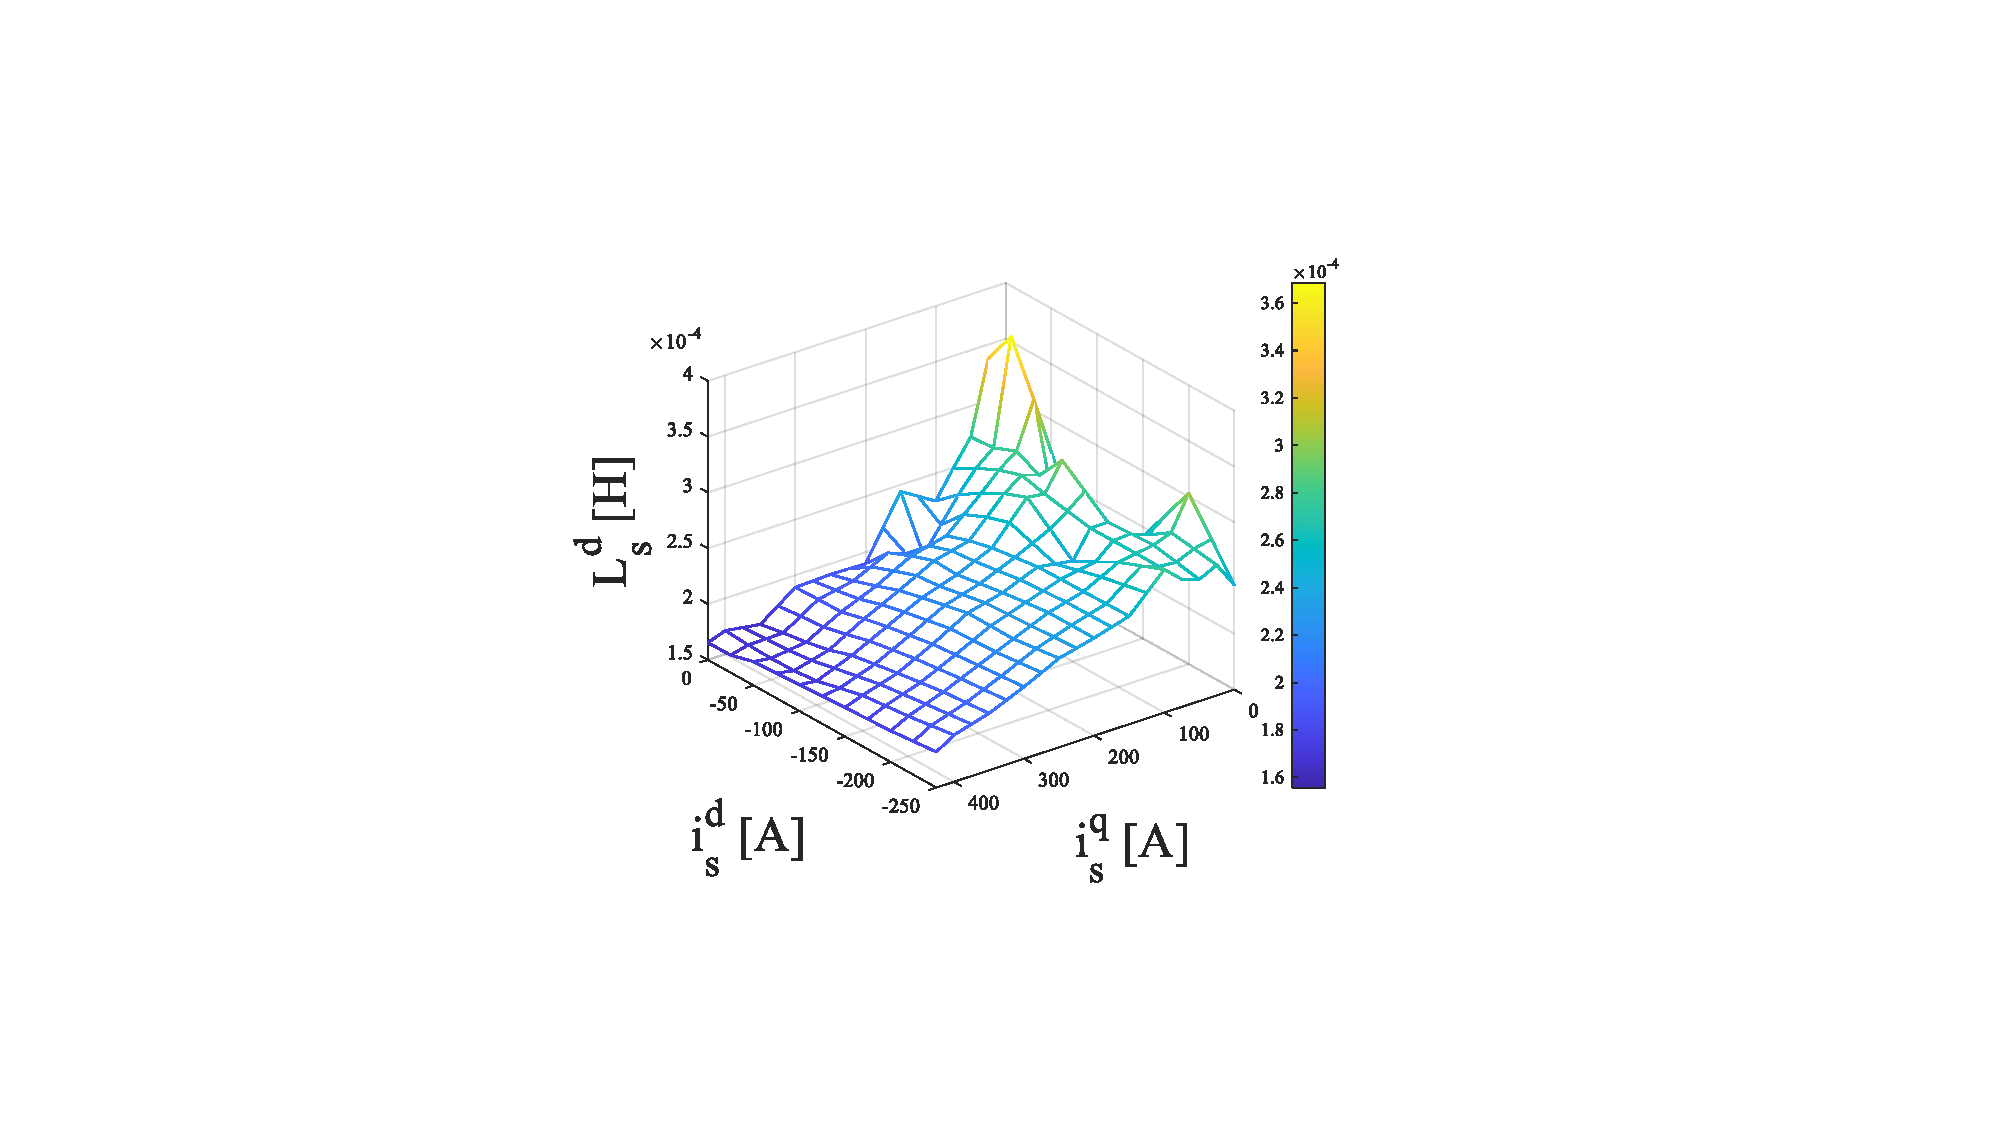
\includegraphics[scale=0.4]{chapters/Fig2.4a.pdf}
        \caption{}
        \label{Fig:2.4a}
    \end{subfigure}
    \hfill
    \begin{subfigure}[b]{0.30\textwidth}
        \centering
        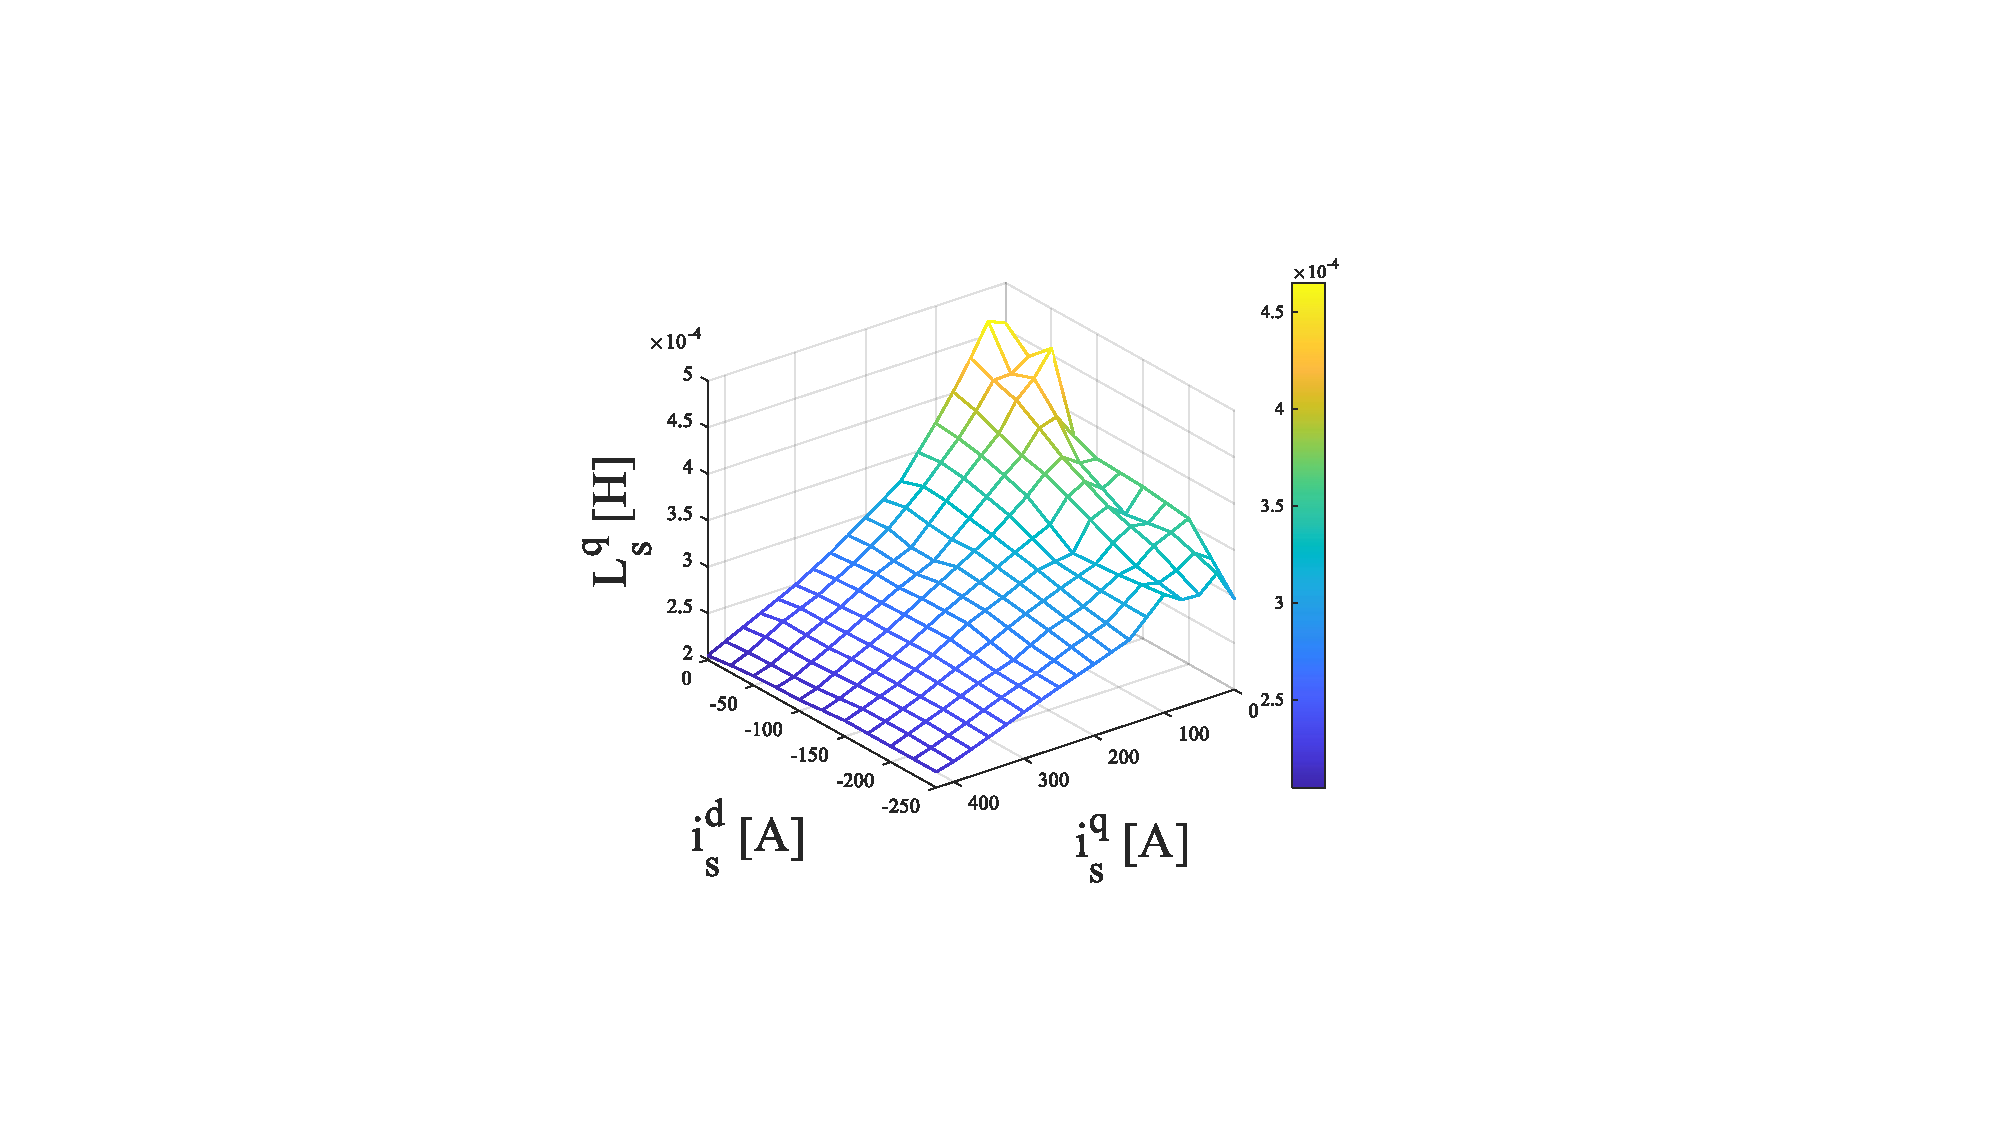
\includegraphics[scale=0.4]{chapters/Fig2.4b.pdf}
        \caption{}
        \label{Fig:2.4b}
    \end{subfigure}
    \hfill
    \begin{subfigure}[b]{0.30\textwidth}
        \centering
        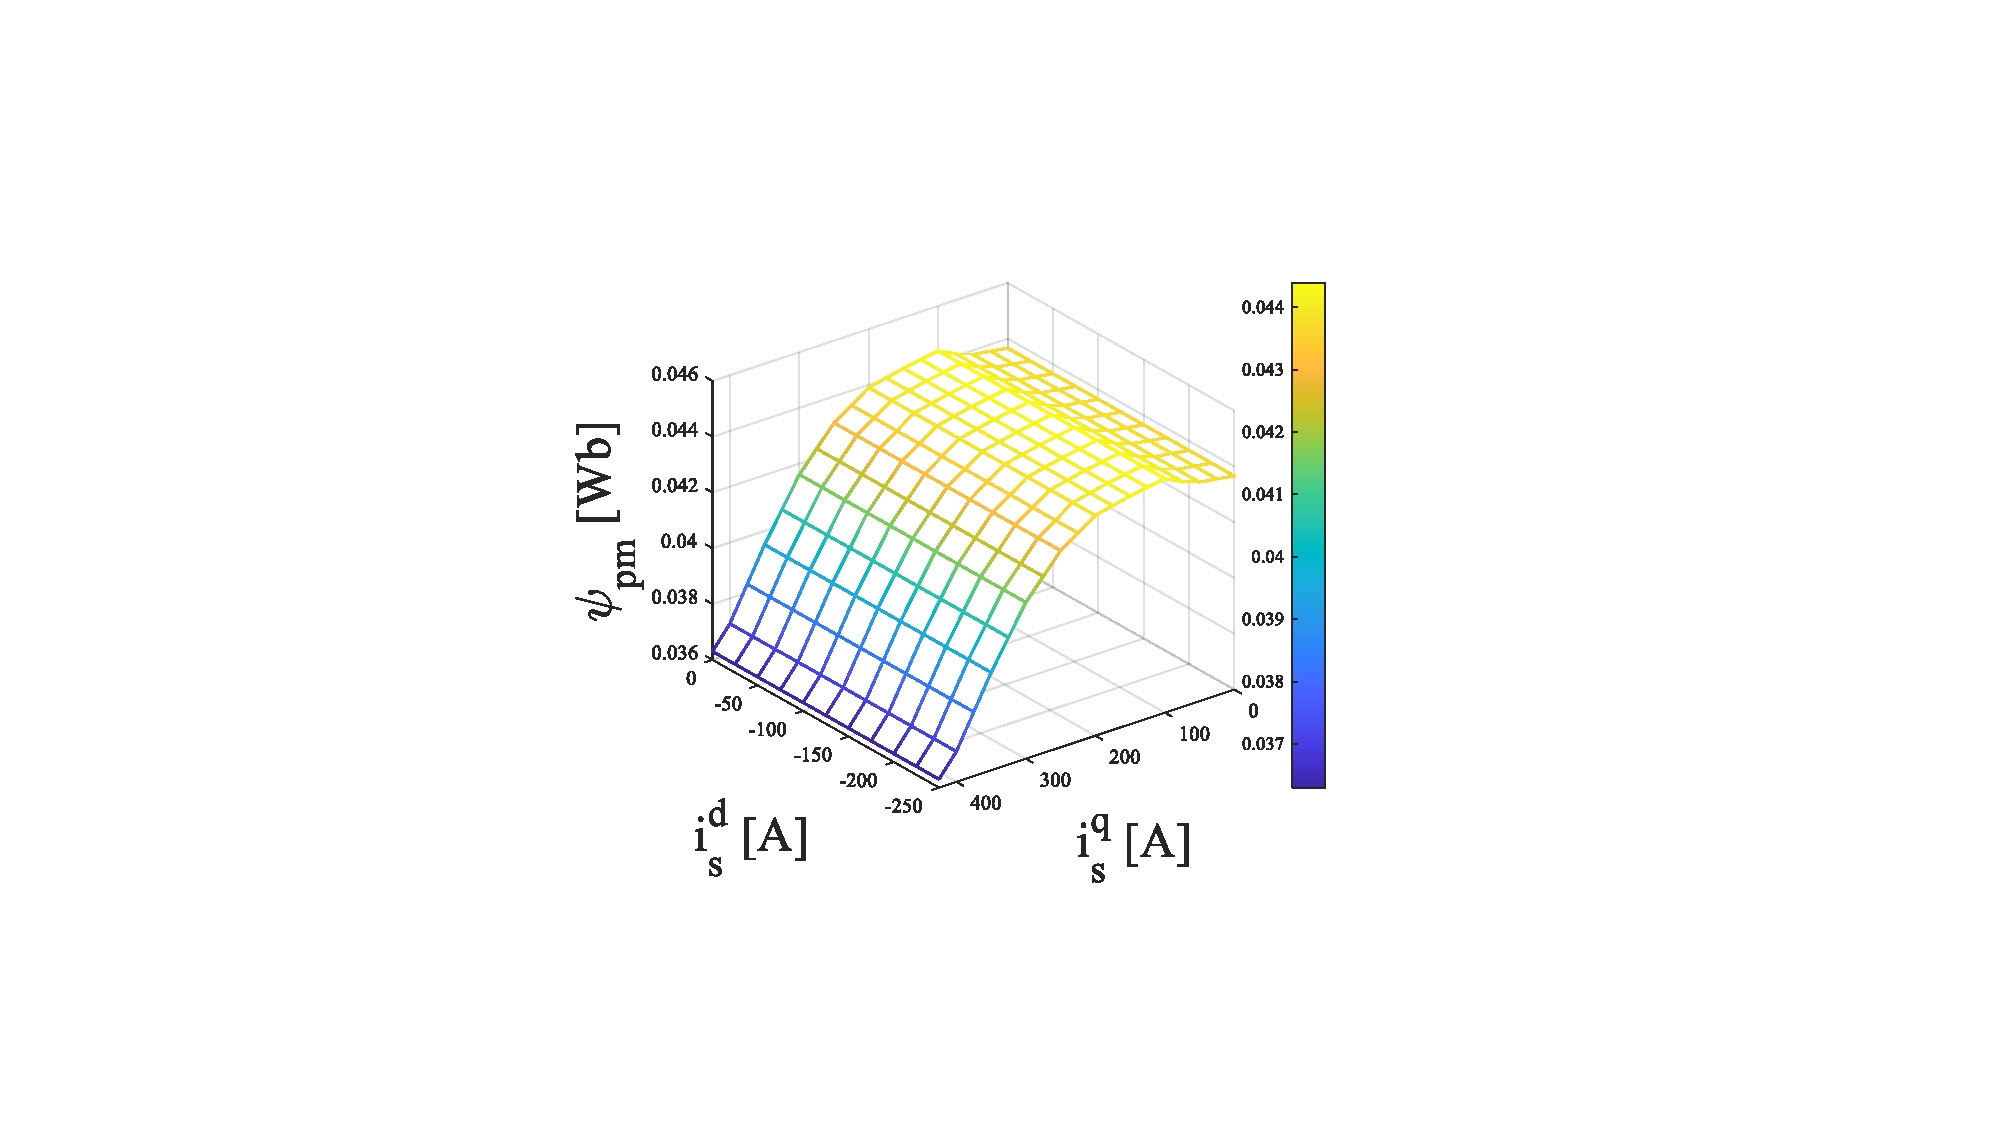
\includegraphics[scale=0.4]{chapters/Fig2.4c.pdf}
        \caption{}
        \label{Fig:2.4c}
    \end{subfigure}
    \caption{Stator inductance and permanent magnetic flux linkage of a PMSM versus $d-$ and $q$-axes currents. (a) d-axis inductance. (b) q-axis inductance. (c) permanent magnetic flux linkage.}
    \label{Fig:2.4}
\end{figure}

Practically, the machine parameters ($L^d_s$, $L^q_s$, $\psi_{pm}$) are highly influenced by the temperature of the cores (stator, rotor), permanent magnets in the rotor and stator winding, which degrades the permeability of the cores and reduces their ability to magnetize \cite{k1},\cite{k2}. Ultimately, due to continuous changes in parameters caused not only by the behavior of the stator current but also by temperature variations in the rotor and stator windings, it is necessary to develop methods for online estimation of these parameters to improve the operating performance of the SMs.

\section{Optimal Control Strategy for SM}\label{chap2:2.2} 
Model Predictive Control (MPC) offers a more flexible optimal control solution compared to conventional feedforward-based PI regulators that determine the switch mode operation of power switch devices through PWM (Pulse Width Modulation), by evaluating an appropriate cost function that allows to selection of the possible switching states as control inputs from either a Continuous Control Set (CCS) or a Finite Control Set (FCS). This approach offers the advantage of optimizing several control conditions such as switching frequency, switching losses, and machine torque ripple minimization while considering the constraints of the SM. However, to achieve these optimizations, a significant computation burden is required, especially because the CCS-MPC method determines control inputs within a continuous control set range, necessitating complex and computationally intensive optimization \cite{c2.2_5},\cite{c2.2_6}. In contrast, the FCS-MPC method considers control inputs within a finite control set, simplifying the optimization process and reducing the computational burden compared to CCS-MPC. Moreover, FCS-MPC has the advantages of intuitive concept, easy handling of nonlinear constraints, and realization of multivariable control \cite{c2.2_1},\cite{c2.2_2}.
Additionally, the calculation burden of the optimal solutions for MPC-based methods has been improved by the development of cost-effective and efficient microprocessors, allowing for extensive computations at low cost \cite{c2.2_3}. Therefore, with accurate parameter information of the SMs model, the FCS-MPC method is an excellent alternative to PI regulator. This section focuses on introducing the FCS-MPC method for the current control of IPMSM.

\subsubsection{Finite Control Set Model Predictive Current Control} \label{sec2:2-2}
Finite Control Set Model Predictive Current Control (FCS-MPCC) is an FCS-MPC-based optimal current control method that defines the objective function as the error between the predicted current and the reference current, based on discrete-time model dynamics. The switching states (one of the eight switching states of a 2-level inverter) corresponding to the minimum value of this objective function are determined as the control inputs. Therefore, it has the advantage of easily designing and evaluating objective functions to optimize control conditions such as switching and power loss minimization while considering the voltage and current limits of the synchronous machine.

Typically, to obtain the predicted currents, the derivative of the $d$-$q$ axis currents with respect to discrete time can be expressed using a \emph{forward Euler approximation} \cite{c2.2_3} as follows.
\begin{equation}\label{eqn:2.15}
\frac{d\mathbf{i}^{dq}_s}{dt} \approx \frac{\mathbf{i}^{dq}_s(k+1) - \mathbf{i}^{dq}_s(k)}{T_s},
\end{equation}
Here, \( T_s \) is the sampling time. 

By substituting the discrete-time current dynamics in (\ref{eqn:2.15}) into the scalar equations (\ref{eqn:2.12}) and (\ref{eqn:2.13}) respectively, the prediction of the future currents in the ($d$,$q$)-reference frame at the \( k+1 \) time can be expressed as 
\begin{align}\label{eqn:2.16}
i^{d,p}_s(k + 1) &= \left( 1 - \frac{R_s T_s}{L^d_s} \right) i^{d}_s(k) + \frac{T_s}{L^d_s}\left( \omega_r(k) L^q_s i^{q}_s(k) + {u_{s}^q}^*(k)  \right),  \\\label{eqn:2.17} 
i^{q,p}_s(k + 1) &= \left( 1 - \frac{R_s T_s}{L^q_s} \right) i^{q}_s(k) - \frac{T_s}{L^q_s}\left( \omega_r(k) L^d_s i^d_s(k) + \omega_r(k) \psi_{pm}  - {u_{s}^d}^*(k) \right),
\end{align}
where $i^{d,p}_s$ and $i^{q,p}_s$ represent the predicted $d$- and $q$-axis stator currents. Here, the possible voltage references in the ($d$,$q$)-reference frame as control inputs (${u_{s}^d}^*$,${u_{s}^q}^*$) are composed of a finite control set (8 switching states). Accordingly, to determine the control inputs (${u_{s}^d}^*$,${u_{s}^q}^*$), the three-phase voltage references in the ($a$,$b$,$c$)-reference frame can be expressed using the switching functions as follows
\begin{align}\label{eqn:2.18}
{u_{s}^a}^*(n) &= \frac{U_{dc}}{3}\left(2S_a(n) - S_b(n) - S_c(n)\right), \\\label{eqn:2.19}
{u_{s}^b}^*(n) &= \frac{U_{dc}}{3}\left(2S_b(n) - S_a(n) - S_c(n)\right), \\\label{eqn:2.20}
{u_{s}^c}^*(n) &= \frac{U_{dc}}{3}\left(2S_c(n) - S_b(n) - S_a(n)\right), \\
\bm{S}(n) &= \left(S_a(n),S_b(n),S_c(n)  \right), 
\end{align}
where \( U_{dc} \) is the input voltage, and \( {u_{s}^a}^* \), \( {u_{s}^b}^* \), and \( {u_{s}^c}^* \) denote the voltage references in the ($a$,$b$,$c$)-reference frame, respectively. \( S_a \), \( S_b \), and \( S_c \) represent the switching states of each phase, where $1$ indicates the switch is ON and $0$ indicates the switch is OFF, operating complementarily within each phase's switch leg and \(\bm{S}\) denotes the switching state vector, including each phase. Table \ref{Table:2.1} and Fig.\ref{Fig:2.8} show all possible combinations of the switching states, space voltage vectors, and cost functions. 

\begin{table}[t]
\centering
\setlength{\tabcolsep}{5pt}
\begin{tabular}{    c|
    c|
    c|c|c|c
}
\toprule
\hline
\multicolumn{1}{c|}{Cost Function} & \multicolumn{1}{c|}{Switching States} & \multicolumn{3}{c}{Phase Voltages} & \multicolumn{1}{|c}{Space Voltage Vectors} \\
\hline
$g$ &$\mathbf{S}(n)$ = ($S_a$,$S_b$,$S_c$) & $u^a_{s}$ & $u^b_{s}$ & $u^c_{s}$ & $\mathbf{U}_n(n =0-7)$\\  
\hline
$g_0$ & $\mathbf{S}(0)$ = ($0$,$0$,$0$) & $0$ & $0$ & $0$ & $\mathbf{U}_0 =0\angle 0^\circ$ \\
$g_1$ &  $\mathbf{S}(1)$ = ($1$,$0$,$0$) & $\frac{2}{3}U_{dc}$ & $-\frac{1}{3}U_{dc}$ & $-\frac{1}{3}U_{dc}$ & $\mathbf{U}_1 =\frac{2}{3}U_{dc}\angle 0^\circ$\\
$g_2$ &  $\mathbf{S}(2)$ = ($1$,$1$,$0$) & $\frac{1}{3}U_{dc}$ & $\frac{1}{3}U_{dc}$ & $-\frac{2}{3}U_{dc}$ & $\mathbf{U}_2 =\frac{2}{3}U_{dc}\angle 60^\circ$\\
$g_3$ & $\mathbf{S}(3)$ = ($0$,$1$,$0$) & $-\frac{1}{3}U_{dc}$ & $\frac{2}{3}U_{dc}$ & $-\frac{1}{3}U_{dc}$ & $\mathbf{U}_3 =\frac{2}{3}U_{dc}\angle 120^\circ$ \\
$g_4$ & $\mathbf{S}(4)$ = ($0$,$1$,$1$) & $-\frac{2}{3}U_{dc}$ & $\frac{1}{3}U_{dc}$ & $\frac{1}{3}U_{dc}$ & $\mathbf{U}_4 =\frac{2}{3}U_{dc}\angle 180^\circ$ \\
$g_5$ & $\mathbf{S}(5)$ = ($0$,$0$,$1$) & $-\frac{1}{3}U_{dc}$ & $-\frac{1}{3}U_{dc}$ & $\frac{2}{3}U_{dc}$ & $\mathbf{U}_5 =\frac{2}{3}U_{dc}\angle 240^\circ$\\
$g_6$ &  $\mathbf{S}(6)$ = ($1$,$0$,$1$) & $\frac{1}{3}U_{dc}$ & $-\frac{2}{3}U_{dc}$ & $\frac{1}{3}U_{dc}$ & $\mathbf{U}_6 =\frac{2}{3}U_{dc}\angle 300^\circ$\\
$g_7$ &  $\mathbf{S}(7)$ = ($1$,$1$,$1$) & $0$ & $0$ & $0$ & $\mathbf{U}_7 =0\angle 0^\circ$\\
\hline
\bottomrule
\end{tabular}
\caption{Switching states, phase 
 voltages and space voltage vector with a cost function.}\label{Table:2.1}
\end{table}
\begin{figure}[t]
    \centering
    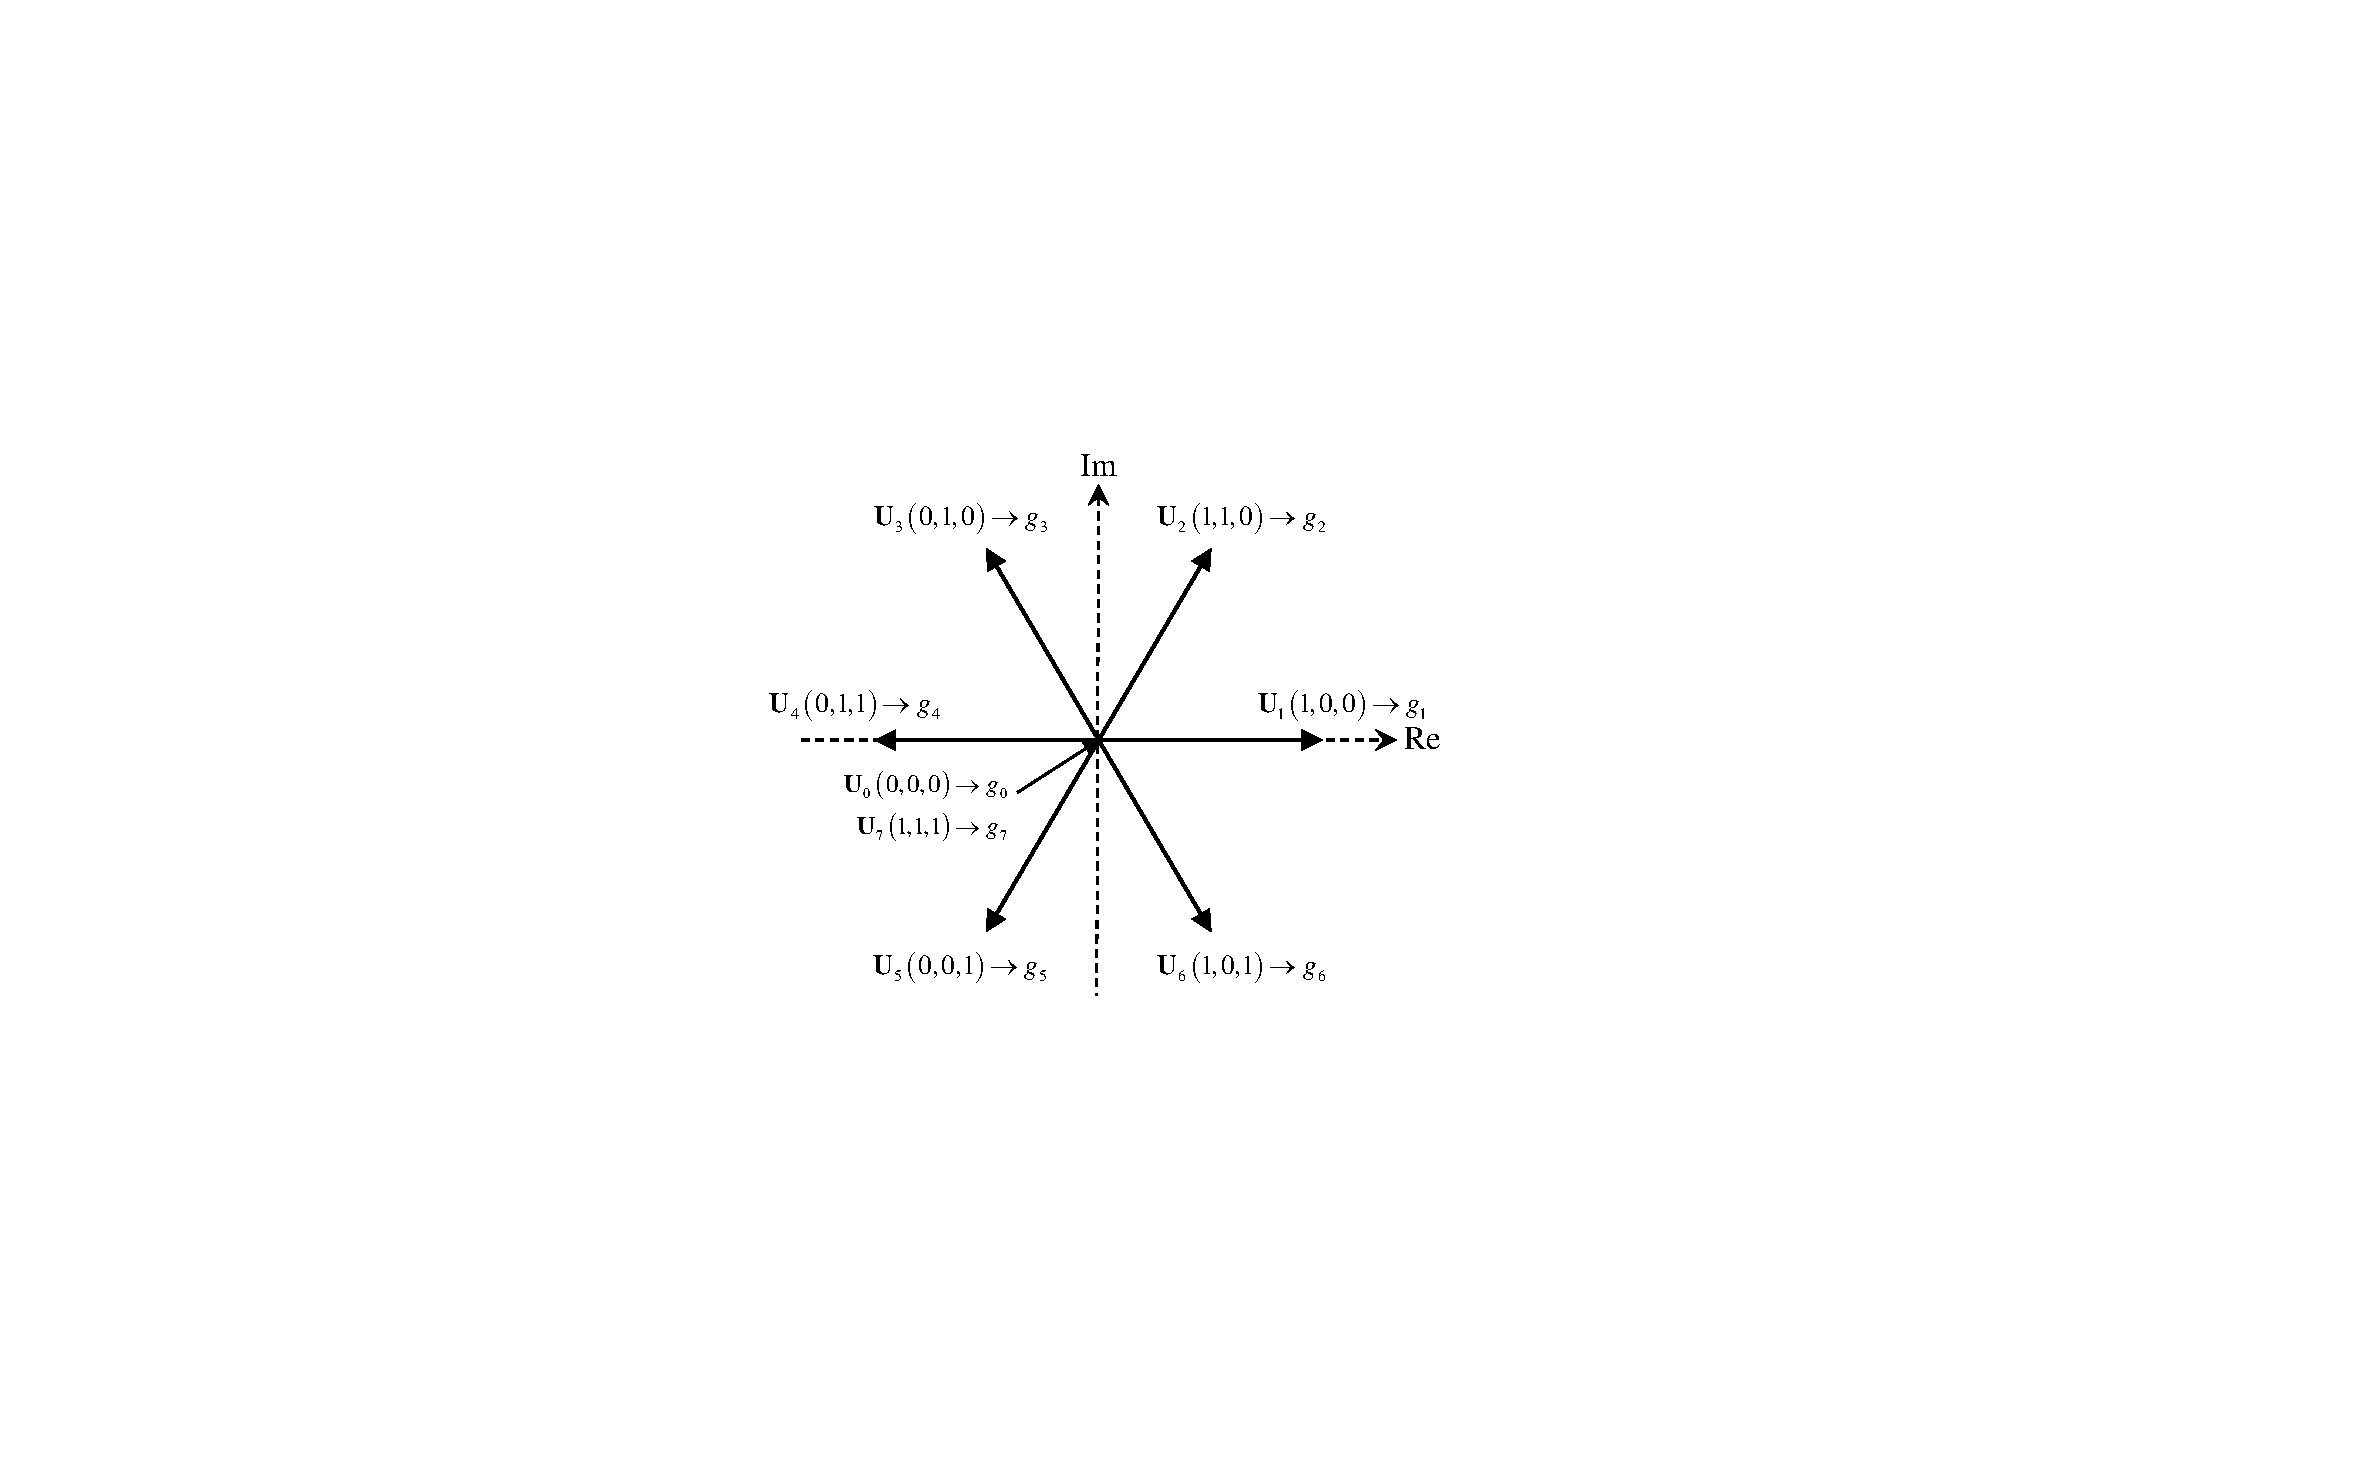
\includegraphics[scale=0.70]{chapters/Fig2.8.pdf}
    \caption{Voltage vectors and corresponding cost function in the complex plane.}
    \label{Fig:2.8}
\end{figure}

Transforming the voltage references in the ($a$,$b$,$c$)-reference frame (${u_{s}^a}^*$,${u_{s}^b}^*$,${u_{s}^c}^*$) to the ($d$,$q$)-reference frame (${u_{s}^d}^*$,${u_{s}^q}^*$) results as follows
\begin{align}\label{eqn:2.22}
{u_{s}^d}^*(k) &= \frac{2}{3} \left( {u_{s}^a}^* \cos\left(\theta_r\right) + {u_{s}^b}^* \cos\left(\theta_r - \frac{2\pi}{3}\right) + {u_{s}^c}^* \cos\left(\theta_r + \frac{2\pi}{3}\right) \right), \\\label{eqn:2.23}
{u_{s}^q}^*(k) &= -\frac{2}{3} \left( {u_{s}^a}^* \sin\left(\theta_r\right) + {u_{s}^b}^* \sin\left(\theta_r - \frac{2\pi}{3}\right) + {u_{s}^c}^* sin\left(\theta_r + \frac{2\pi}{3}\right) \right),
\end{align}
whereby substituting the voltage references in (\ref{eqn:2.22}) and (\ref{eqn:2.23}) calculated from the three-phase stator voltage references (${u_{s}^a}^*$,${u_{s}^b}^*$,${u_{s}^c}^*$) for the 8 switching states into the predicted current dynamics in (\ref{eqn:2.16}) and (\ref{eqn:2.17}), all the predicted currents can be obtained. Therefore, to determine the voltage references in the ($d$,$q$)-reference frame that minimizes the errors between the current references and the predicted currents, the objective function can be derived and evaluated, which the switching state of minimum cost functions $g$ for 8 all switching states are determined as the control input voltages. The operating principle of predictive current control for the implementation is shown in Algorithm \ref{Algorithm:2.1} and Fig \ref{Fig:2.6} shows the control scheme based on the FCS-MPC current controller. 

\begin{figure}[t]
    \centering
    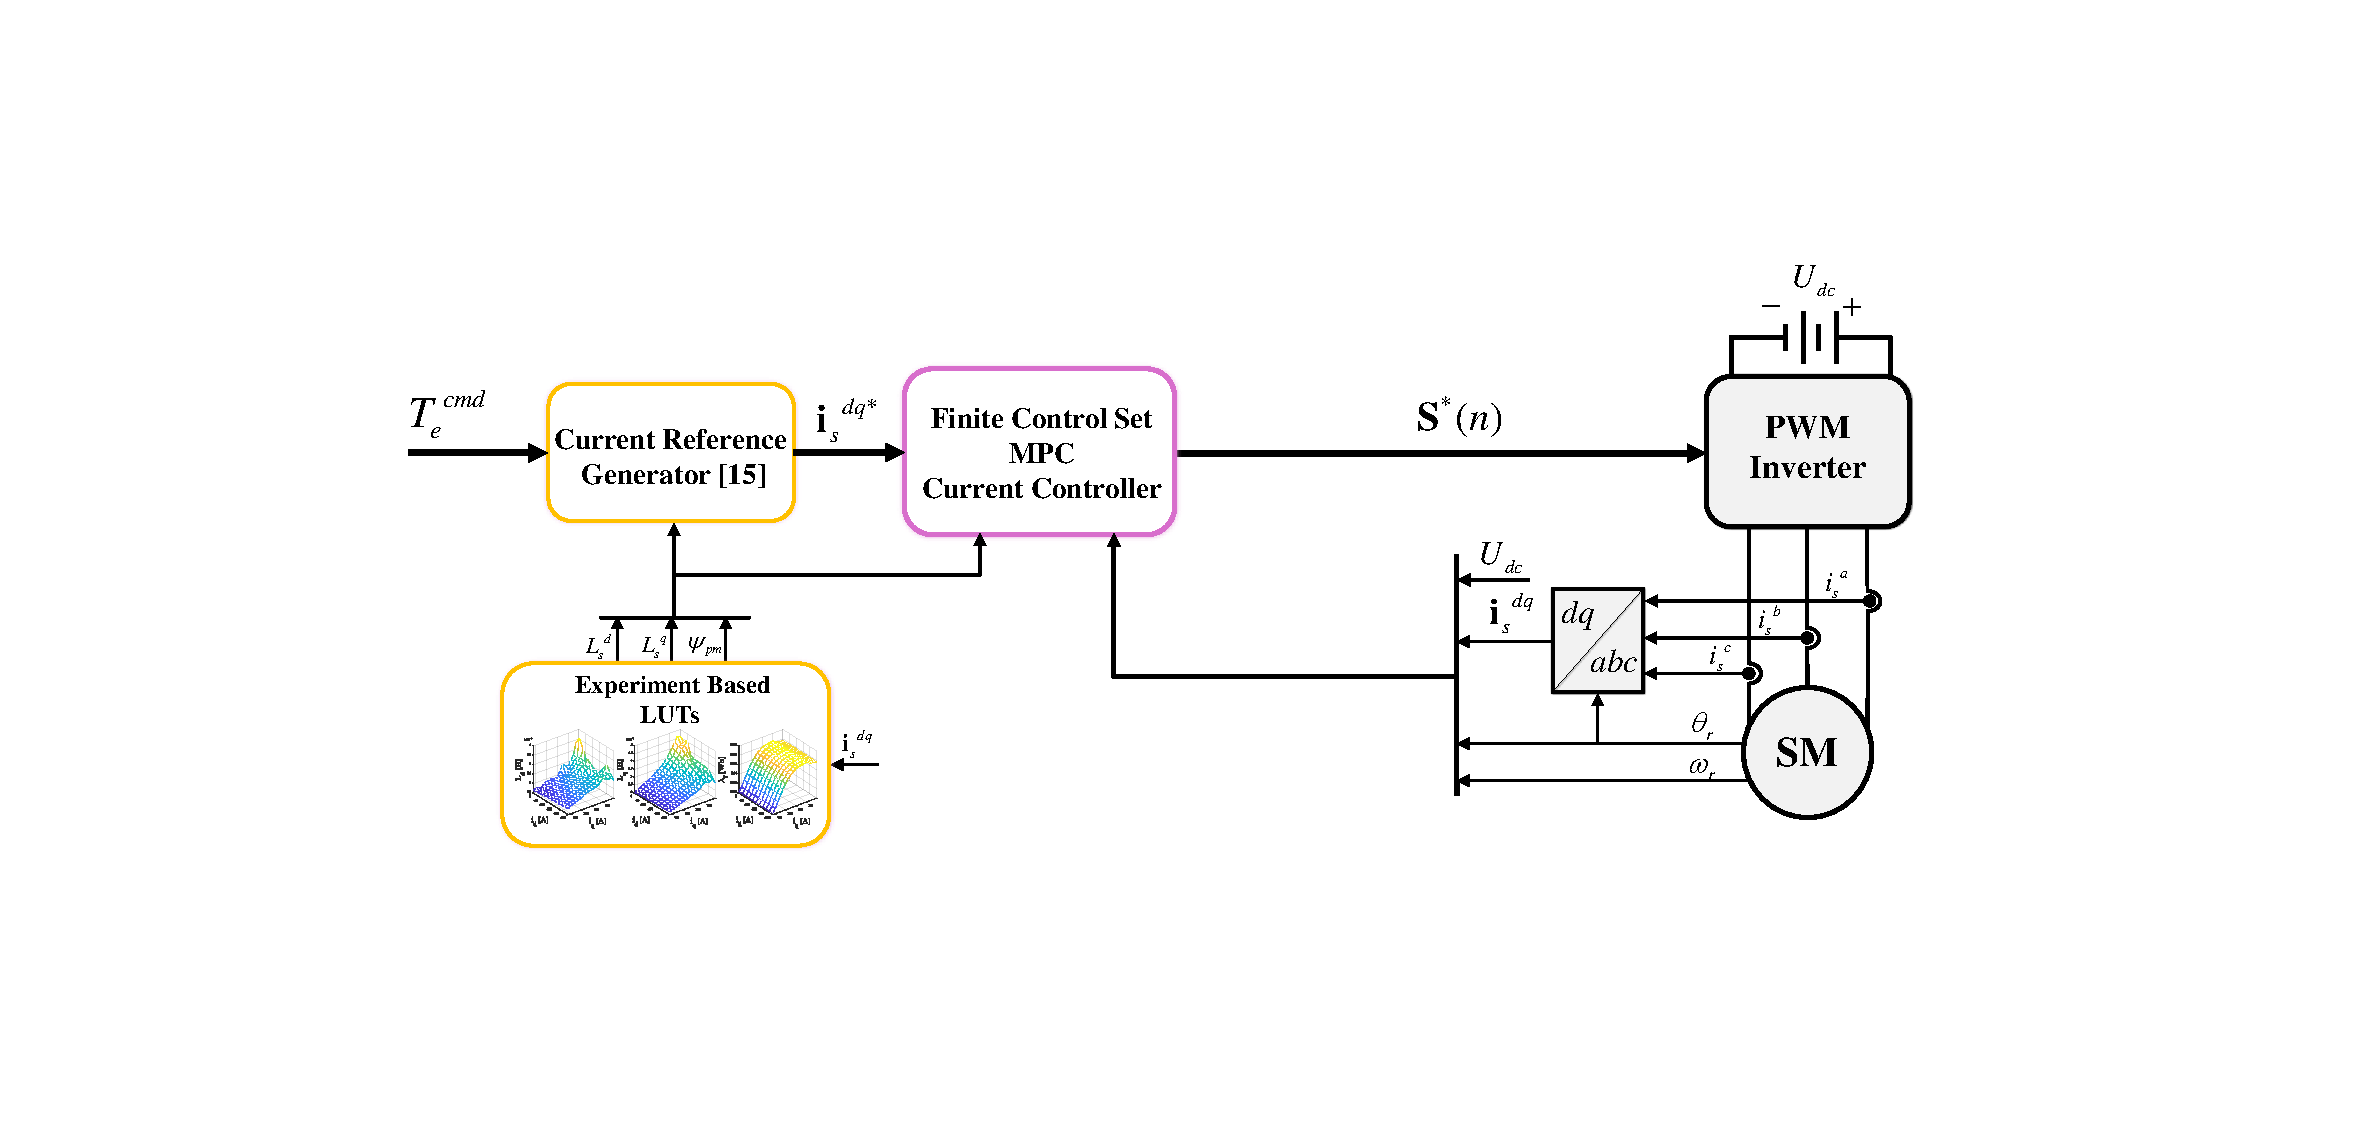
\includegraphics[scale=0.6]{chapters/Fig2.6.pdf}
    \caption{Control scheme using FCS-MPC current controller.}
    \label{Fig:2.6}
\end{figure}
\begin{algorithm}[!]
\caption{Predictive current control algorithm}
\begin{algorithmic}[1]
\STATE \textbf{Startup}
\STATE Measure $i_{dq}(k)$ and $\omega_r(k)$
\STATE $n = 0$
\FOR{$n \leq 7$}
\STATE $n = n + 1$
\STATE Calculate $\mathbf{u}^*_{dq}(k) \leftarrow {u_{s}^a}^*(n),{u_{s}^b}^*(n),{u_{s}^c}^*(n)$ using (\ref{eqn:2.18})$-$(\ref{eqn:2.20})
\STATE Predict $\mathbf{i}_{dq}(k+1)$ using (\ref{eqn:2.16}) and (\ref{eqn:2.17})
\STATE Evaluate cost function $g = |i_{d}^* - i_{d}^p| + |i_{q}^* - i_{q}^p|$
\STATE Store optimal values for $g$
\ENDFOR
\IF{$n = 7$}
    \STATE Apply the optimal space voltage vector $\mathbf{u}^*_n$ for minimum $g$
\ENDIF
\RETURN $\mathbf{u}^*_{dq}(k)$
\STATE Wait for next sampling instant
\end{algorithmic}\label{Algorithm:2.1}
\end{algorithm}
\begin{equation}\label{eqn:2.24}
g = \left| i_{d}^* - i_{d}^p \right| + \left| i_{q}^* - i_{q}^p \right|
\end{equation}

The accuracy of the predicted currents through FCS-MPCC is highly influenced by the machine parameters (inductance, stator, and permanent magnet flux linkages) \cite{c2.2_4}. However, as previously mentioned, machine parameters are not only nonlinear functions of stator currents but also very sensitive to temperature changes in the stator and rotor cores, as well as the stator windings and permanent magnets. Therefore, for robust control of FCS-MPCC, it is essential to develop a flux estimator or parameter identifier that can estimate and update the mismatched parameters in the prediction model online, thereby improving the accuracy of the predicted model.

\section{Existing Flux Linkage Estimators}\label{chap2:2.3} 
As mentioned above, online information on the machine parameters is essential not only for improving the operating performance of SMs (such as SM fault diagnosis, MTPA, etc.) but also for achieving robust optimal control of the predictive model, especially the FCS-MPCC method. However, it is extremely challenging to directly estimate all machine parameters using only the two current dynamics in (\ref{eqn:2.12}) and (\ref{eqn:2.13}) due to rank deficiency in the model equations (to estimate more than three parameters with only two equations) \cite{c2.3_3}. Therefore, instead of directly estimating the machine parameters, the stator flux linkage is first estimated \cite{c1_1},\cite{c2.3_4},\cite{c2.3_5},\cite{c2.3_6}, and then machine parameter identification is conducted online \cite{c2.3_1} or offline \cite{c2.3_2}. This section introduces existing methods for stator flux linkage estimation as a preliminary step for machine parameters estimation.

\subsection{Steady-State Assumption-based Flux Linkage Estimator} \label{sec2:2.3.1}
The machine dynamic model in (\ref{eqn:2.9}) can be rearranged as a flux-based dynamic model
\begin{align}\label{eqn:2.25}
\frac{d}{dt} \bm{\psi}^{dq}_s(t) = \mathbf{u}^{dq}_s(t) - R_s \mathbf{i}^{dq}_s(t) - \omega_r(t) \mathbf{J} \bm{\psi}^{dq}_s(t),
\end{align}
where the $d$-$q$ axis flux linkage vectors are constant in steady state, making the time derivative of the flux vector zero. Therefore, based on the steady-state assumption, the flux estimate vector can be simplified as
\begin{align}\label{eqn:2.26}
\bm{\hat \psi}^{dq}_s(s) = \frac{1}{\omega_r} \mathbf{J}^{-1} \left( \mathbf{u}^{dq*}_{s}(s) - \hat{R}_s \mathbf{i}^{dq}_s(s) \right),
\end{align}
where \(\hat{R}_s\) is the estimated stator resistance, which is a nonlinear function of the stator winding temperature but is assumed to be accurately estimable, and \(\bm{\hat{\psi}}^{dq}_s\) represents the estimate of the flux linkage vector. The electrical angular velocity \(\omega_r\) can be assumed to be constant because it is sufficiently slow compared to the electrical signals. The control input voltages \( u^{dq*}_{s} \) obtained from FCS-MPCC in (\ref{eqn:2.22}) and (\ref{eqn:2.23}) contain significant switching frequency components, so a low pass filter (LPF) is applied to filter out these high-frequency components, resulting in the flux estimate vector
\begin{align}\label{eqn:2.27}
\bm{\hat \psi}^{dq}_{s,\text{LPF}}(s) = \frac{\omega_\text{LPF}}{s + \omega_\text{LPF}} \bm{\hat \psi}^{dq}_s(s),
\end{align}
where \( \omega_\text{LPF} \) is the LPF cutoff frequency. 

This approach allows for the easy derivation of \(d\)- and \(q\)-axis flux estimates based on the steady state, so it is commonly used in many industries to obtain the parameters needed to create experiment-based lookup tables (LUTs). However, during transient states, this method produces significant estimation errors resembling spikes, distorts the magnitude and phase due to the cut-off frequency of the LPF, and is especially unsuitable for low-speed regions \cite{c2.3_7}, \cite{c2.3_8}, making it inappropriate for online estimation.

\subsection{Voltage and Current Model-based Flux Linkage Estimator} \label{sec2:2.3.2}
\subsubsection{Voltage Model}
The machine dynamic model in (\ref{eqn:2.5}) can be rearranged as a flux-based dynamic model
\begin{align}\label{eqn:2.28}
\frac{d}{dt}\bm{\psi}^{\alpha\beta}_s(t) = \mathbf{u}^{\alpha\beta}_s(t) - R_s \mathbf{i}^{\alpha\beta}_s(t),
\end{align}
which is defined as the \emph{voltage model} \cite{c2.1_1} for the flux linkage estimation. By purely integrating the voltage model in (\ref{eqn:2.28}), the flux estimate vector can be derived as follows 
\begin{align}\label{eqn:2.29}
\bm{\psi}^{\alpha\beta}_{s,\text{int}}(t) = \int_{0}^{t} \left( \bm{u}^{\alpha\beta*}_{s}(\tau) - \hat R_s \bm{i}^{\alpha\beta}_s(\tau) \right) d\tau + \bm{\psi}^{\alpha\beta}_{s,\text{int}}(0),
\end{align}
where \(\bm{{\psi}}^{\alpha\beta}_{s,{\text{int}}}:=({\psi}^{\alpha}_{s,{\text{int}}},{\psi}^{\beta}_{s,{\text{int}}})^\top\) is the integration result of the voltage model and \(\bm{{\psi}}^{\alpha\beta}_{s,{\text{int}}}(0):=({\psi}^{\alpha}_{s,{\text{int}}}(0),{\psi}^{\beta}_{s,{\text{int}}}(0))^\top\) is the flux estimate vector of the current model is the initial value of the flux vector. However, if there are errors in the input voltages $\bm{u}^{\alpha\beta*}_{s}$ and initial value $\bm{\psi}^{\alpha\beta}_{s,\text{int}}(0)$, or if sensor biases or inverter nonlinearities are present, the flux estimate obtained from simple integration will contain estimation errors (DC offset). 

To filter out the low-frequency DC offset components, a high-pass filter (HPF) is commonly applied to the flux estimate vector
\begin{align}\notag
\bm{\hat{\psi}}^{\alpha\beta}_{s,v}(s) &= \frac{s}{s + \omega_\text{HPF}} \times \frac{1}{s}\times\left[  \bm{u}^{\alpha\beta*}_{s}(s) - \hat{R}_s \bm{i}^{\alpha\beta}_{s}(s)\right]\\\label{eqn:2.37}
&= \frac{1}{s + \omega_\text{HPF}} \times \left[  \bm{u}^{\alpha\beta*}_{s}(s) - \hat{R}_s \bm{i}^{\alpha\beta}_s(s)\right]
\end{align}
in the S-domain \cite{c2.3_9}, \cite{c2.3_10}, where \(\bm{\hat{\psi}}^{\alpha\beta}_{s,{v}}:=(\hat{\psi}^{\alpha}_{s,{v}},\hat{\psi}^{\beta}_{s,{v}})^\top\) is the flux estimate vector of the voltage model and \(\omega_{\text{HPF}}\) is the cutoff frequency of the HPF.

While this approach performs well at high speeds (only in steady state), it becomes sensitive to filter gain settings near the cutoff frequency of the HPF, especially in low-speed regions, significantly distorting the magnitude and phase of the estimates.

\subsubsection{Current Model}
The flux linkage model in (\ref{eqn:2.10}) is defined as the \emph{current model} \cite{c2.1_1} and this flux vector is represented by the nominal inductance $\mathbf{{L}}^{dq}_{s,0}$ and permanent flux $\bm{{\psi}}^{dq}_{pm,0}$
\begin{align}\label{eqn:2.31}
\bm{\hat{\psi}}^{dq}_{s,i} &= \mathbf{{L}}^{dq}_{s,0}\mathbf{i}^{dq}_s
+ \bm\psi_{pm,0}, \quad 
 \mathbf{{L}}^{dq}_{s,0} = \begin{bmatrix}
{L}^d_{s,0} & 0 \\
0 & {L}^q_{s,0} \\
\end{bmatrix}, {\bm{{\psi}}^{dq}_{pm,0} = \begin{bmatrix}
{\psi_{pm,0}} \\
0
\end{bmatrix}},
\end{align}
where \(\bm{\hat{\psi}}^{dq}_{s,{i}}:=(\hat{\psi}^{q}_{s,{i}},\hat{\psi}^{q}_{s,{i}})^\top\) is the flux estimate vector of the current model in the ($d$,$q$)-reference frame.

This approach provides relatively robust flux estimation in low-speed and low-current regions. However, it cannot deal with the inaccuracies of machine parameters caused by magnetic saturation and temperature variations in permanent magnets, resulting in estimation errors.

\subsubsection{Hybrid Model}\begin{figure}[t]
    \centering
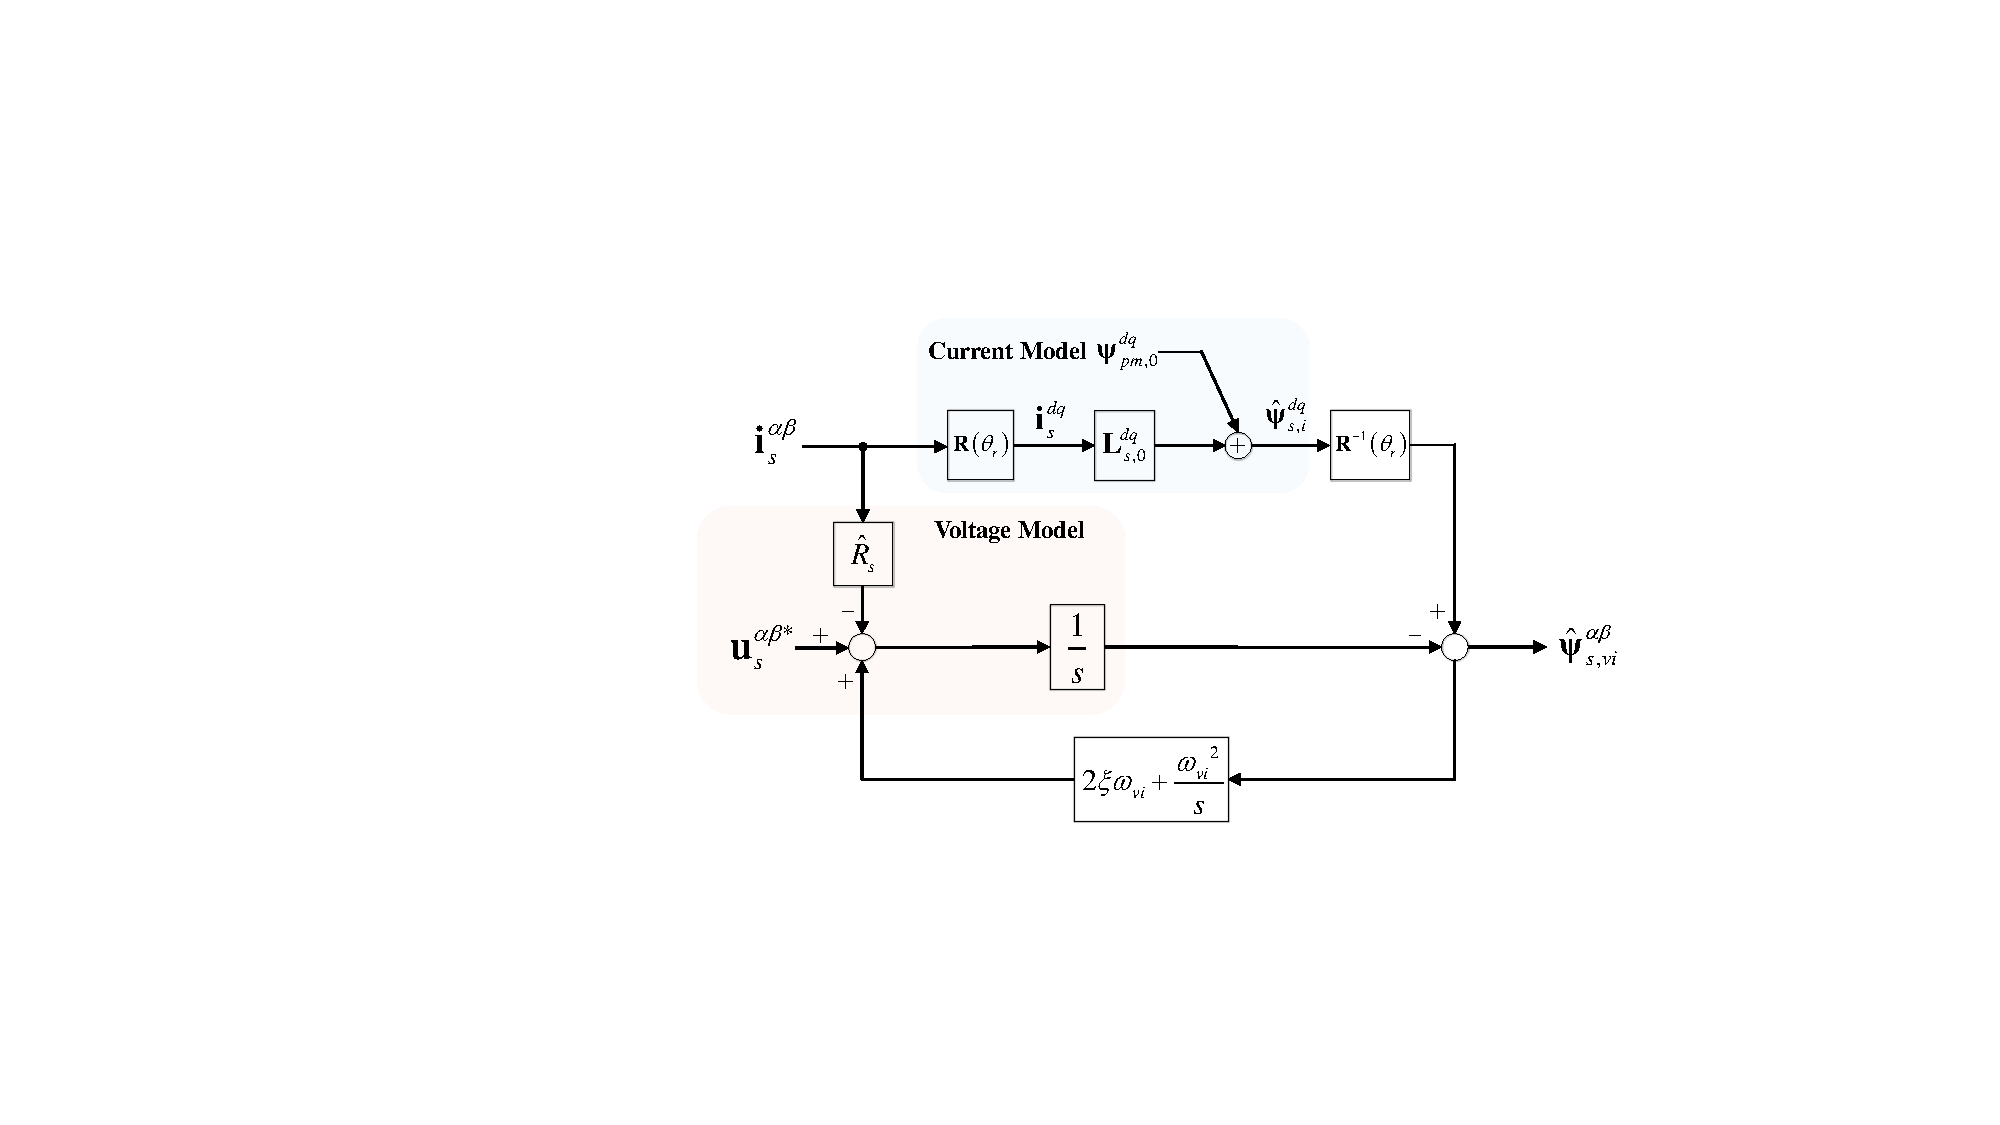
\includegraphics[scale=0.8]{chapters/Fig2.9.pdf}
    \caption{Block diagram of the voltage and current model-based flux linkage estimator.}
    \label{Fig:2.9}
\end{figure}
To overcome the disadvantages of the aforementioned voltage and current models, a Gopinath-style observer has been proposed, which uses the current model in low-speed regions and the voltage model in high-speed regions \cite{c2.3_11}, \cite{c2.3_12}, \cite{c2.3_13}, \cite{c2.3_14}. This observer uses a proportional-integral (PI) filter to smoothly transition between the flux estimates of the two models near the crossover frequency. The flux linkage estimate vector
\begin{align}\label{eqn:2.32}
\bm{\hat{\psi}}^{\alpha\beta}_{s,{vi}}(s)
=
\frac{s^2}{s^2 + 2 \xi \omega_{vi} s + \omega_{vi}^2}\bm{\hat{\psi}}^{\alpha\beta}_{s,v}(s) +
\frac{2 \xi \omega_{vi} s + \omega_{vi}^2}{s^2 + 2 \xi \omega_{vi} s + \omega_{vi}^2}\bm{R}^{-1}(\theta_r)\bm{\hat{\psi}}^{dq}_{s,i}(s)
\end{align}
in the ($\alpha$,$\beta$)-reference frame can be derived, where \(\bm{\hat{\psi}}^{\alpha\beta}_{s,{vi}}:=(\hat{\psi}^{\alpha}_{s,{vi}},\hat{\psi}^{\beta}_{s,{vi}})^\top\) represents the flux estimate vector of the voltage-current hybrid model, and \(\xi\) and \(\omega_{\text{vi}}\) denote the damping ratio and the natural frequency of the PI filter, respectively. Figure \ref{Fig:2.9} shows the block diagram of the flux observer based on the conventional voltage and current models.

Although this approach can be used to estimate flux linkages over a wide operating range, variations in the nominal parameters used in the current model can lead to a substantial decrease in estimation performance, especially during transient states. To address these drawbacks and ensure robustness against parameter variations, a modified flux observer for the voltage-current-based estimation model was presented in \cite{c2.3_15}, where the flux linkage errors caused by parameter inaccuracies can be determined by the output of the integral controller at steady state. 

However, this approach can significantly degrade estimation performance at low speeds because the reciprocal of the rotor speed affects the flux estimates. Additionally, there has been insufficient research on improving estimation performance during transient states, and there is a lack of information on selecting the cutoff frequency for the PI filter. Without precise criteria for filter design, phase, and magnitude distortions can occur in the estimates, significantly affecting estimation performance, especially during transient states. 

\subsection{Disturbance Observer-based Flux Linkage Estimator \cite{c1_1}}\label{chap2:2.3.3}
The novel approach of estimating nonlinear flux linkages in the time domain using a disturbance observer-based state observer was introduced in \cite{c1_1}. This estimator is very simple and highly effective for nonlinear flux linkage estimation. The key idea is to separate the $d$-$q$ axis flux linkage vector in (\ref{eqn:2.10}) into a linear term $\mathbf{L}_{s,0}\mathbf{i}^{dq}_{s}$ and a nonlinear flux linkage term $\Delta\boldsymbol{\psi}^{dq}_s(\mathbf{i}^{dq}_s)$, i.e.
\begin{align}\label{eqn:2.33}
\bm{\psi}^{dq}_s(t) = \mathbf{L}^{dq}_{s,0} \mathbf{i}^{dq}_s(t) + \underbrace{\left( \mathbf{L}^{dq}_{s} - \mathbf{L}^{dq}_{s,0} \right) \mathbf{i}^{dq}_s(t) + \boldsymbol{\psi}^{dq}_{pm}}_{=:\Delta{\boldsymbol{\psi}^{dq}_s}(\mathbf{i}^{dq}_s)=\Delta{\boldsymbol{\psi}^{dq}_s}(t)} \xLeftrightarrow{\hspace{0.5cm}} \ \mathbf{i}^{dq}_s(t) = {\mathbf{L}^{dq}_{s,0}}^{-1}\left(\bm{\psi}^{dq}_s(t) - \Delta{\boldsymbol{\psi}^{dq}_s}(t)\right)
\end{align}
with constant (but arbitrarily) nominal (static) inductance matrix $\mathbf{L}^{dq}_{s,0} \in \mathbb{R}^{2\times 2}$ and nonlinear flux vector $\Delta\boldsymbol{\psi}^{dq}_s:=(\Delta{\psi}^{d}_s,\Delta{\psi}^{q}_s)^\top$, including cross-coupling and saturation effects. 
The time derivative of the nonlinear flux linkage in (\ref{eqn:2.33})
\begin{align}\label{eqn:2.34}
\frac{d}{dt}\Delta{\boldsymbol{\psi}^{dq}_s} = \underbrace{\mathbf{\dot L}^{dq}_{s} \mathbf{i}^{dq}_s + \left( \mathbf{L}^{dq}_{s} - \mathbf{L}^{dq}_{s,0} \right) \mathbf{\dot i}^{dq}_s + \boldsymbol{\dot \psi}^{dq}_{pm}}_{=:\mathbf{d}^{dq}_s(\mathbf{i}^{dq}_s,\mathbf{\dot i}^{dq}_s) = \mathbf{d}^{dq}_s(t)}
\end{align}  
can be derived, where the lumped disturbance vector $\mathbf{d}^{dq}_s:=(d^{d}_s,d^{q}_s)^\top$ can be expressed as a nonlinear function of the current $\mathbf{i}^{dq}_s$ and the derivative of the current $\mathbf{\dot i}^{dq}_s$. Since it is very difficult to know the exact model for these disturbance signals, the physical behaviors of the dynamics in (\ref{eqn:2.34}) can be explained by the following assumption.

\textbf{Assumption (A.2.1)} The dynamics system in (\ref{eqn:2.9}) are bounded-input-bounded-output (BIBO) stable and the lumped disturbance vector in (\ref{eqn:2.34}) is upper bounded by
\begin{equation}\notag
   ||\mathbf{d}^{dq}_s|| \stackrel{(\ref{eqn:2.34})}\leq  ||\mathbf{\dot L}^{dq}_{s}|| ||\mathbf{i}^{dq}_s|| +  ||\mathbf{L}^{dq}_{s} - \mathbf{L}^{dq}_{s,0}||  ||\mathbf{\dot i}^{dq}_s|| + ||\boldsymbol{\dot \psi}^{dq}_{pm}||.
\end{equation}
\textbf{Assumption (A.2.2)}
All parameters and signals in the ($d$,$q$)-reference frame in (\ref{eqn:2.33}) become constant in steady state (i.e. constant current and speed), so the nonlinear flux linkage $\Delta\boldsymbol{\psi}^{dq}_s$ has the characteristics
\begin{equation}\notag
    \Delta\boldsymbol{\psi}^{dq}_s(t) = \left( \mathbf{L}^{dq}_{s} - \mathbf{L}^{dq}_{s,0} \right) \mathbf{i}^{dq}_s(t) + \boldsymbol{\psi}^{dq}_{pm} = \mathbf{c}^{dq}_s,
\end{equation}
with unknown but constant $\mathbf{c}^{dq}_s:=(c^{d}_s,c^{q}_s)^\top$ and their time derivatives become zero vector (only) in steady state. Therefore, the disturbance vector $\mathbf{d}^{dq}_s $ in (\ref{eqn:2.34}) becomes the zero vector \(\mathbf{O}_2\), i.e. 
\begin{align}\notag
    \mathbf{d}^{dq}_s \rightarrow \mathbf{O}_2 \quad \left(
    \mathbf{\dot L}^{dq}_{s}\rightarrow \mathbf{O}_{2\times2}, \mathbf{\dot i}^{dq}_s \rightarrow \mathbf{O}_2, \boldsymbol{\dot \psi}^{dq}_{pm} \rightarrow \mathbf{O}_2 \text{ as } t \rightarrow \infty 
    \right)
\end{align}
which means that these disturbance signals can be assumed to be step signals.

Substituting (\ref{eqn:2.33}) into (\ref{eqn:2.9}) leads to the altered dynamic model
\begin{equation}
\begin{aligned}\label{eqn:2.35}
\begin{cases}
\frac{d}{dt}{\bm{\psi}}^{dq}_s(t) = \mathbf{u}^{dq}_s(t) - R_s {\mathbf{L}^{dq}_{s,0}}^{-1} \left( \bm{\psi}^{dq}_s(t) - \Delta{\boldsymbol{\psi}^{dq}_s}(t) \right) - \omega_r(t) \mathbf{J} \bm{\psi}^{dq}_s(t) \\
\frac{d}{dt}{\Delta}{\boldsymbol{\psi}^{dq}_s}(t) = \mathbf{d}^{dq}_s(t) \\
\mathbf{i}_{dq}(t) = {\mathbf{L}^{dq}_{s,0}}^{-1} \left( \bm{\psi}^{dq}_s(t) - \Delta{\boldsymbol{\psi}^{dq}_s}(t) \right)
\end{cases}
\end{aligned}.
\end{equation}
By defining the nonlinear flux linkage vector $\Delta{\boldsymbol{\psi}^{dq}_s}$ as an extended state to be estimated, the state-space model is expressed as
\begin{equation}\label{eqn:2.36}
\left\{
\begin{aligned}
\frac{d}{dt}\mathbf{x}(t) &= \mathbf{A}(\omega_r)\mathbf{x}(t) + \mathbf{B}\mathbf{u}(t) + \mathbf{d}(t) \\
\mathbf{y}(t) &= \mathbf{C}\mathbf{x}(t)
\end{aligned}
\right.
\end{equation}
with 
\begin{equation*}
\begin{aligned}
\mathbf{x} &:= \begin{pmatrix} \bm{\psi}^{dq}_s \\ \Delta{\boldsymbol{\psi}^{dq}_s} \end{pmatrix}, \quad \mathbf{u} := \mathbf{u}^{dq}_s, \quad \mathbf{y} := \mathbf{i}^{dq}_s, \quad \mathbf{O}_{2\times2} := \begin{bmatrix}
0  & 0\\
0 & 0
\end{bmatrix}, \quad \mathbf{I}_{2\times2} := \begin{bmatrix}
1  & 0\\
0 & 1
\end{bmatrix}, \\
\mathbf{A}(\omega_r) &:= \begin{bmatrix}
-R_s {\mathbf{L}^{dq}_{s,0}}^{-1}-\omega_r \mathbf{J}  & R_s {\mathbf{L}^{dq}_{s,0}}^{-1}\\
\mathbf{O}_{2\times2} & \mathbf{O}_{2\times2}
\end{bmatrix}, \quad \mathbf{B} := \begin{bmatrix}
\mathbf{I}_{2\times2} \\
\mathbf{O}_{2\times2}
\end{bmatrix}, \quad \mathbf{C} := \begin{bmatrix}
{\mathbf{L}^{dq}_{s,0}}^{-1} & -{\mathbf{L}^{dq}_{s,0}}^{-1}
\end{bmatrix}, \\
\mathbf{d} &:= \begin{bmatrix}
    \mathbf{O}_2 & \mathbf{d}^{dq}_s
\end{bmatrix}^\top, \quad \mathbf{O}_2 := \begin{bmatrix}
    0 & 0
\end{bmatrix}^\top,
\end{aligned}
\end{equation*}
where $\mathbf{x}$ represents the state vector, $\mathbf{u}$ denotes the input vector, $\mathbf{y}$ represents the output vector and $\mathbf{d}$ is the lumped disturbance vector. The matrix $\mathbf{A}(\omega_r)$ is the system matrix with respect to $\omega_r$, $\mathbf{B}$ is the input matrix, and $\mathbf{C}$ is the output matrix. 

To verify if the dynamic system in (\ref{eqn:2.36}) is in an observable form for constant speed $\omega_r$, the observability matrix 
\begin{equation}\label{eqn:2.37}
\mathbf{\mathcal{O}}(\omega_r) = \begin{bmatrix}
\mathbf{C} \\
\mathbf{CA}(\omega_r) \\
\mathbf{CA}(\omega_r)^2 \\
\mathbf{CA}(\omega_r)^3
\end{bmatrix}
\end{equation}
needs to be examined; since the matrix in (\ref{eqn:2.37}) has full rank (i.e., $\mathbf{\mathcal{O}}(\omega_r) = 4$), all states $\mathbf{x}$ can be observed. Accordingly, a linear observer can be designed as follows
\begin{equation}\label{eqn:2.38}
\left\{
\begin{aligned}
\frac{d }{dt}\hat{\mathbf{x}}(t) &= \left[ \mathbf{A}(\omega_r) - \mathbf{F}(\omega_r) \mathbf{C} \right] \hat{\mathbf{x}}(t) + \mathbf{B} \mathbf{u}(t) + \mathbf{F}(\omega_r) \mathbf{y}(t) \\
\hat{\mathbf{y}}(t) &= \mathbf{C} \hat{\mathbf{x}}(t)
\end{aligned},
\right.
\end{equation}
where $\hat{\mathbf{x}}$ and $\hat{\mathbf{y}}$ represent the estimated vector of $\mathbf{x}$ and $\mathbf{y}$, respectively, and $\mathbf{F}(\omega_r) \in \mathbb{R}^{4 \times 2}$ denotes the gain matrix of the observer and depends on the electrical angular speed. To analyze the stability of the estimation convergence, subtracting (\ref{eqn:2.38}) from (\ref{eqn:2.36}) leads to the estimation error dynamics
\begin{equation}\label{eqn:2.39}
\frac{d}{dt}\mathbf{e}(t) = \left[\mathbf{A}(\omega_r) - \mathbf{F}(\omega_r)\mathbf{C}\right] \mathbf{x}(t) - \mathbf{d}(t)
\end{equation}
with the estimation error
\begin{equation}\notag
\mathbf{\tilde x}(t) :=\mathbf{\hat x}(t) - \mathbf{x}(t),
\end{equation}
where \(\mathbf{d} \rightarrow 0\) as \( t \rightarrow \infty \), recalling Assumption (A.2.1) and Assumption (A.2.2). If the gain matrix \(\mathbf{F}(\omega_r)\) is designed such that \(\mathbf{A}-\mathbf{F}(\omega_r)\mathbf{C}\) becomes a stable Hurwitz matrix (i.e., with the desired eigenvalues or poles within the negative complex half-plane), the estimation error \(\mathbf{\tilde{x}}\) will decay exponentially and asymptotically to the equilibrium point. Figure \ref{Fig:2.10} shows the observer block diagrams for DOB-FLE. 
\begin{figure}[t]
    \centering   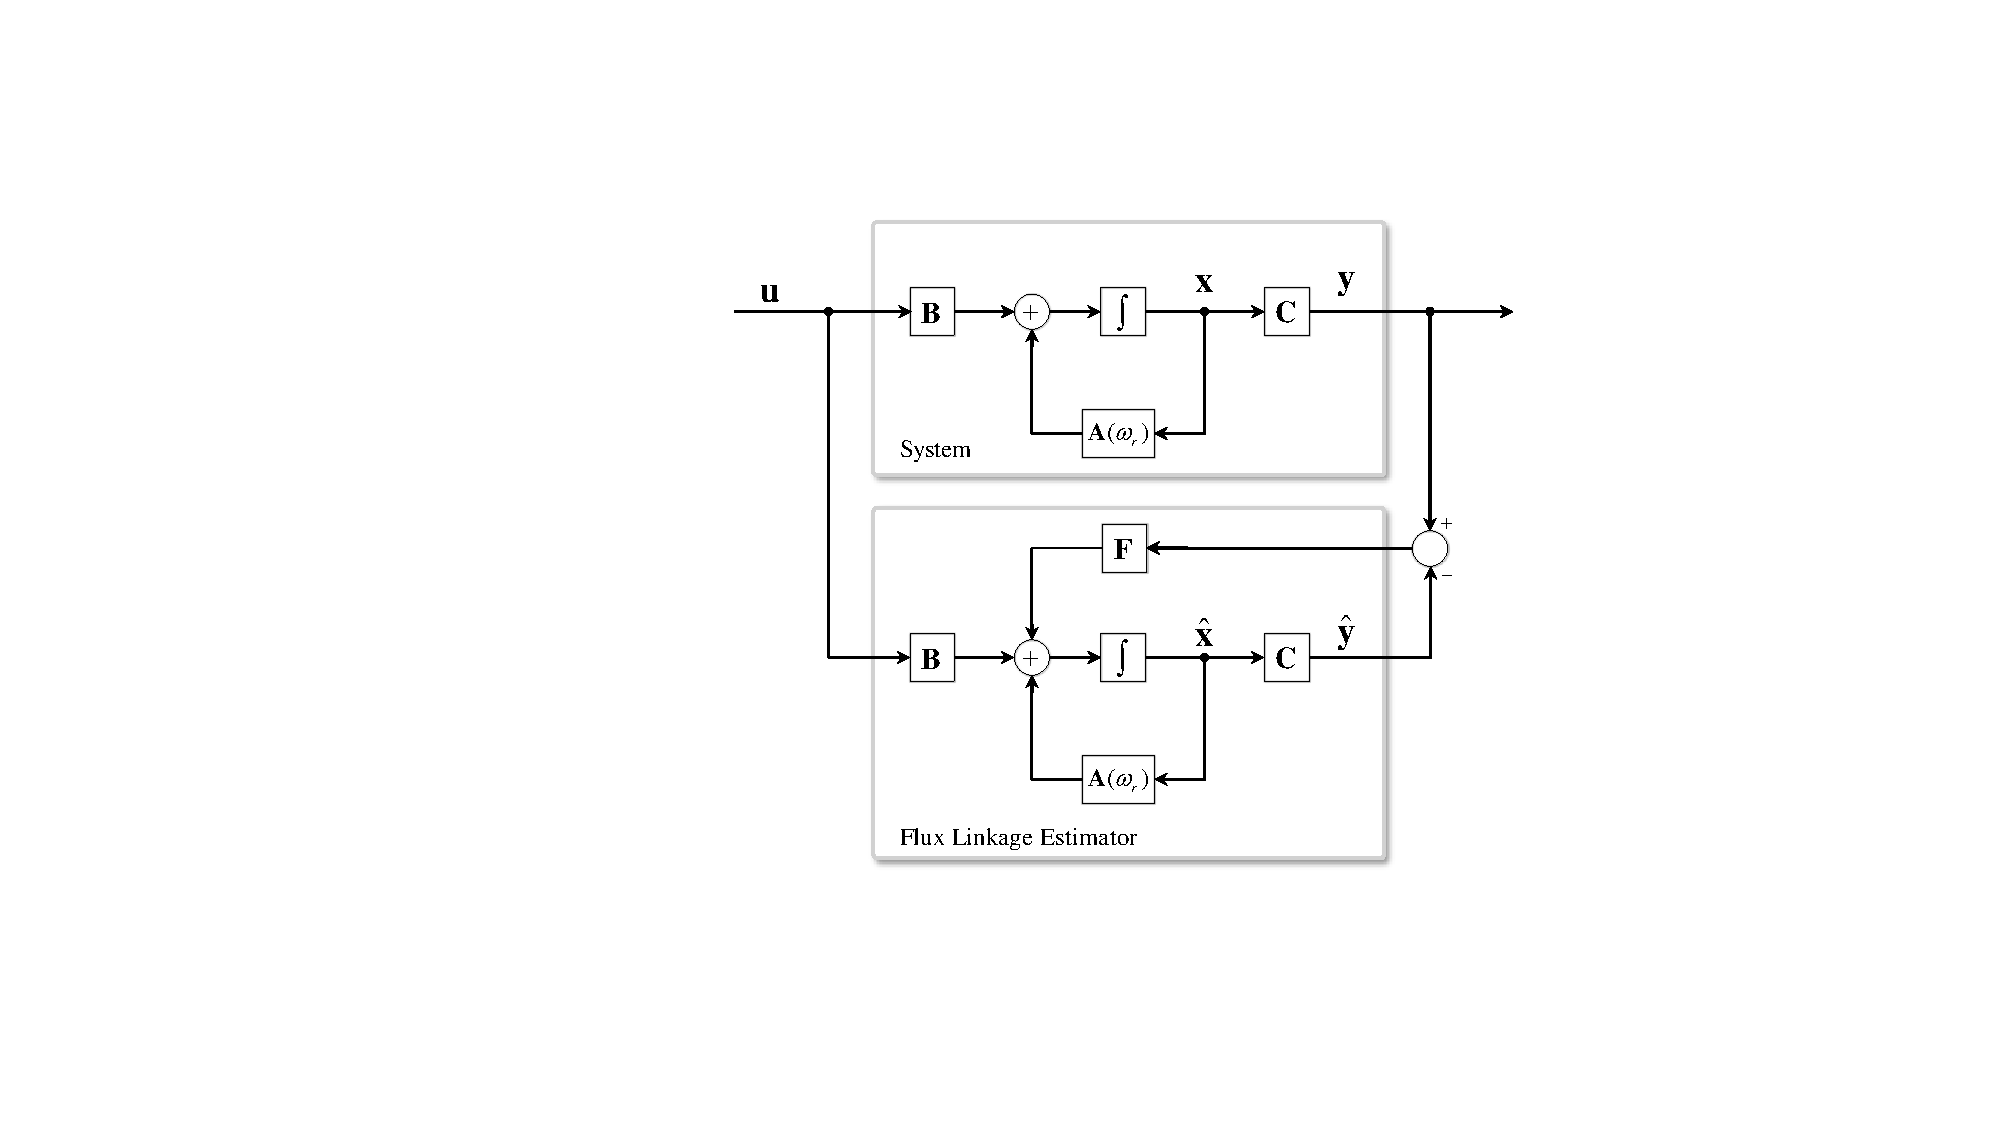
\includegraphics[scale=0.7]{chapters/Fig3.1.pdf}
    \caption{Observer block diagram for DOB-FLE.}
    \label{Fig:2.10}
\end{figure}

DOB-FLE separates the stator flux linkage vector \(\boldsymbol{\psi}^{dq}_s\) into a linear flux with nominal inductance \(\mathbf{L}^{dq}_{s,0}\) and the remaining nonlinear flux term \(\Delta\boldsymbol{\psi}^{dq}_s\), assuming this nonlinear flux term as a constant disturbance signal (i.e. step signal). Therefore, this approach allows for exponential estimation of the nonlinear flux term through a simple linear observer. However, in transient states where the current ramps up or down, the disturbance signals are time-varying with a certain slope rather than constant, causing the magnitude of the disturbance \(\mathbf{d}\) in (\ref{eqn:2.36}) to increase. Additionally, if an inaccurate nominal inductance is used in the observer, the norm of the disturbance vector \(\|\mathbf{d}\|\) increases, leading to significant transient estimation errors.


